% !TeX root = ../main.tex
\chapter{系統實驗與結果討論}\label{chapter:exp}

    本章將說明本研究研究所提出之系統的實作與實驗。
首先說明系統各角色之實作細節,並於接續章節說明實驗與結果討論。


\section{系統實作}\label{sec:impl}

    本章節將說明本研究研究所提出的協定與硬體之實作,包含「會談終端」、「解封伺服器」
與供會談主持者用於與解封伺服器通訊的「行動應用程式」。


\subsection{會談終端}\label{subsec:impl-mbox}

    會談終端包含多個組件,其概念驗證實作硬體組成如圖 \ref{fig:mbox}。

\begin{figure}[H]
    \centering
    \includegraphics[width=1.0\textwidth]{mbox}
    \caption{會談終端概念驗證實作}\label{fig:mbox}
\end{figure}


\paragraph{超音波麥克風干擾器}

    如圖 \ref{fig:mbox} \nameref{fig:mbox}中左下紫色實線多邊形方框所示。
此超音波麥克風干擾器為參考 Yuxin Chen, Huiying Li 等人的實作\cite{chen2020wearable}。
包含一 Arduino Micro 用於產生於$24k\sim26k$之間的偽隨機數與控制周邊裝置。
包含一波形產生器 AD9833,透過SPI與Arduino Micro溝通取得偽隨機數,產生介於$24khz\sim26khz$之間正弦波。
包含一數位放大器 HW-104,用於放大訊號產生器產生的訊號以驅動超音波發射器。
包含一超音波發射器,產生介於$24khz\sim26khz$之間的超音波。
此超音波麥克風干擾器於系統時脈$16Mhz$的單晶片控制器中,每 $2ms$ 產生新的偽隨機數,使其生成干擾超音波。

\paragraph{錄音麥克風}

    如圖 \ref{fig:mbox} \nameref{fig:mbox}中左上黃色實線圓框所示。
包含一USB數位駐極電容式麥克風 Saramonic LavMicro U3A。
用於錄製受超音波麥克風干擾器干擾的會談對話聲音記錄 (\DEFrecJ),
與產生純超音波麥克風干擾器於麥克風的響應輸出(純噪音)之聲音記錄 (\DEFrecN)。

\paragraph{物理控制介面}

    如圖 \ref{fig:mbox} \nameref{fig:mbox}中左上紅色虛線圓框所示。
本系統實作以按鈕為例,提供會談參與者操作與會談終端互動,獲得外部觸發事件,`
用於創建、開始與結束會談。

\paragraph{人機互動介面}

    如圖 \ref{fig:mbox} \nameref{fig:mbox}中右上紅色點虛線方框所示。
本系統實作以電子紙為例,用於傳遞會談的元資料與系統狀態提示給會談主持者與提示系統狀態給會談參與者。
會談主持者透過掃描電子紙螢幕上的 QRCode 接收來自會談終端傳遞的會談的元資料,如圖 \ref{fig:epaper}。
本系統實作按鈕含有一指示燈兼作人機互動介面,於談開始/結束錄音提示系統狀態,如圖 \ref{fig:btn}。

\begin{figure}[H]
    \centering
    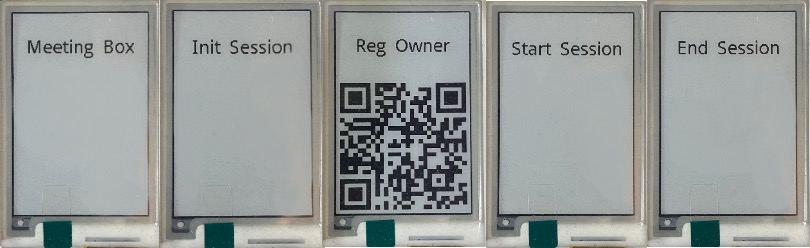
\includegraphics[width=1.0\textwidth]{epaper}
    \caption{電子紙於會談各階段之狀態顯示}\label{fig:epaper}
\end{figure}

\begin{figure}[H]
    \centering
    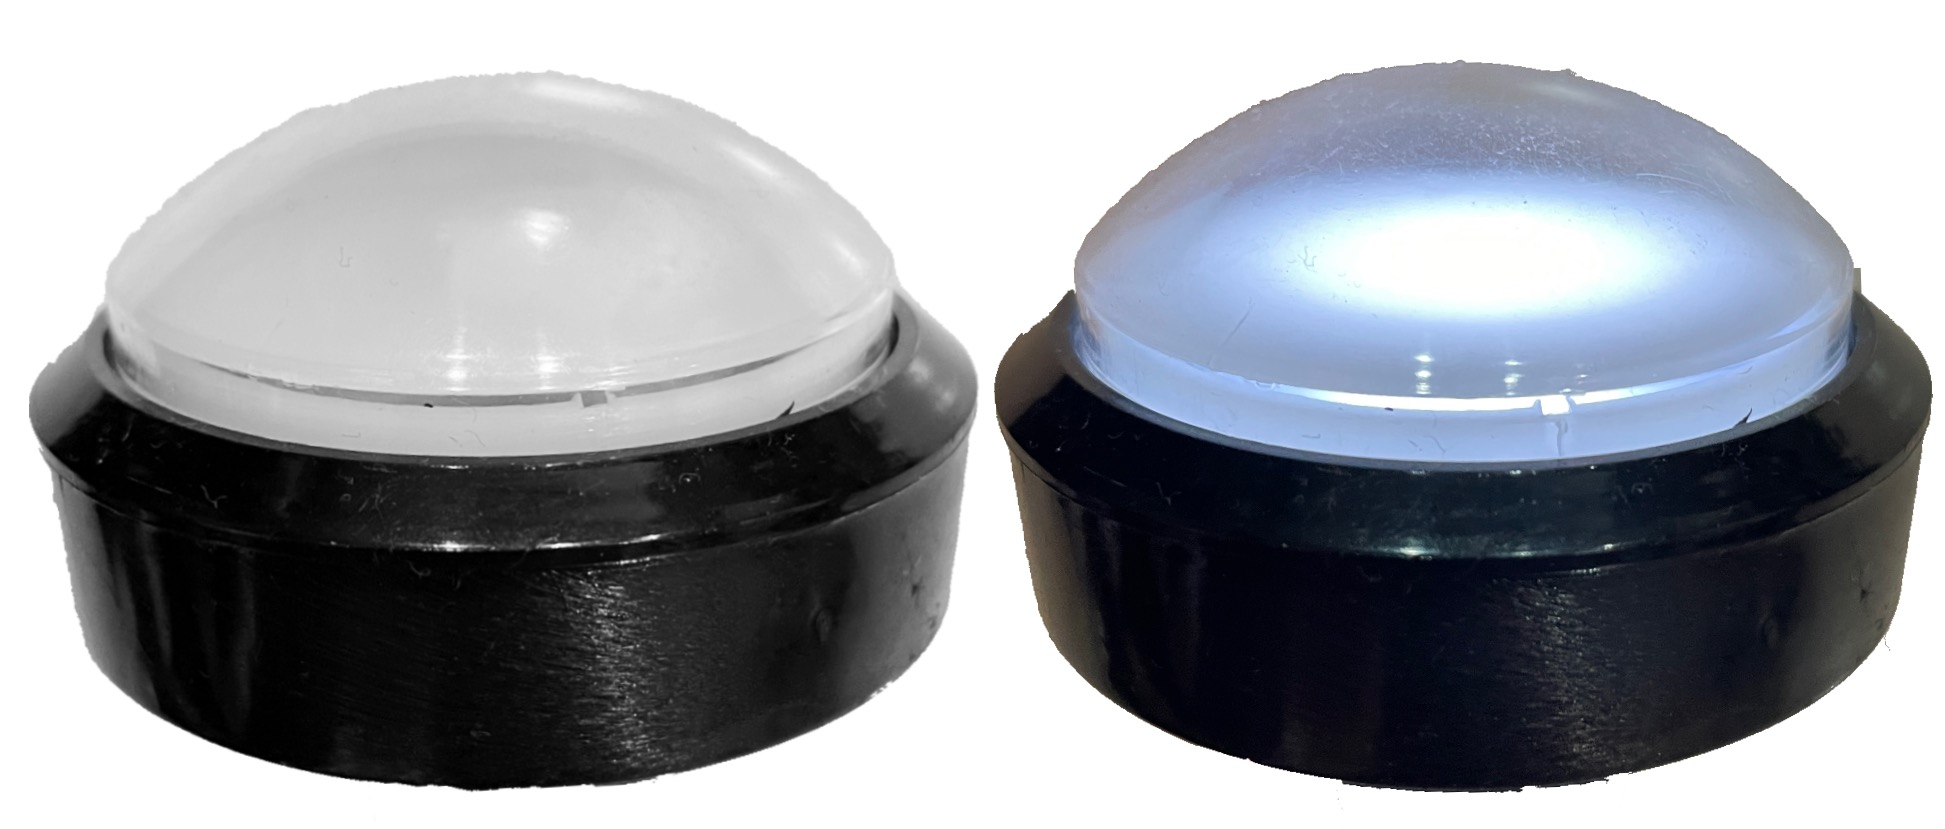
\includegraphics[width=0.5\textwidth]{btn}
    \caption{按鈕於會談開始/結束錄音之狀態指示燈}\label{fig:btn}
\end{figure}

\paragraph{運算控制核心與網路介面}

    如圖 \ref{fig:mbox} \nameref{fig:mbox}中右下綠色點線方框所示。
本系統實作以 Raspberry Pi 4B 為例,包含一 Geekworm X728 電池模組用於供電。
邏輯控制核心使用 Python 實作,控制周邊裝置包含人機互動介面、物理控制介面、超音波麥克風干擾器與錄音麥克風,
並網路介面與解封伺服器溝通。透過 GPIO 接收來自物理控制介面介面的外部觸發事件;透過 SPI 介面控制人機互動介面;
透過 GPIO 控制一外部 MOSFET 開啟關閉超音波干擾器;透過 fork/exec 呼叫 arecord 透過麥克風進行錄音;


\subsection{解封伺服器}\label{subsec:impl-psu}

    本研究所設計之系統中解封伺服器的服務介面由 RESTful\cite{fielding2000architectural} API 組成。
解封伺服器 \DEFserver 中包含6個 API 端點,使用 Golang 搭配 Gin 網頁框架實作。
系統後端解決方案技術架構包含一資料庫 PostgreSQL 13 作為資料關聯綁定以及儲存的媒介;
包含 Docker 容器化執行引擎,用於封裝主動式噪音消除的 Python3 執行環境;
各 API 端點說明如下。

\begin{enumerate}
    \item \texttt{/meeting}

        此 API 端點透過 HTTP 方法 \texttt{POST} 請求,
    為章節 \ref{sec:protocol} \nameref{sec:protocol}中,
    \nameref{subsec:protocol-init-create} 的 $M_{1}$ 、 $M_{2}$ 的實作。
    當 API 端點收到請求後,會執行 \DEFfuncIDgen{} 與 \DEFfuncKgen{},
    分別產生此次會談的唯一識別碼 \DEFsessionID,與此次會談的解封金鑰 \DEFunsealKey。

        其中 \DEFfuncIDgen{} 為唯一識別碼產生函數,其產生須滿足唯一性、隨機性、不可預測性,
    本研究實作以 UUID \cite{rfc4122} 為例。
    \DEFfuncKgen{} 為對稱式加密演算法的金鑰產生函數,
    本研究實作以 AES CFB 模式 \cite{117146}\cite{9171} 為例。

    \item \texttt{/meeting/:id/owner}

        此 API 端點透過 HTTP 方法 \texttt{POST} 請求,
    為章節 \ref{sec:protocol} \nameref{sec:protocol}中,
    \nameref{subsec:protocol-init-reg} 的 $M_{3}^{i}$ 、 $M_{4}^{i}$ 的實作。
    當 API 端點收到請求後,會執行 \DEFfuncPKgen{} 與 \DEFfuncIDgen{},
    分別產生一組屬於會談主持者 \DEFowner 的公開私密金鑰對 $($\DEFpublicKey$,~$ \DEFprivateKey$)$,
    與此會談主持者 \DEFowner 的唯一識別碼 \DEFownerID。

        其中會談主持者的唯一識別碼 \DEFownerID,其產生須滿足唯一性、隨機性、不可預測性,
    本研究實作以 UUID \cite{rfc4122} 為例。
    \DEFfuncPKgen{} 為非對稱加密演算法的公開私密金鑰對產生函數,
    本研究實作以 RSA PKCS\#1 \cite{rfc8017} 為例。
    路由變數 \texttt{:id} 為此次會談的唯一識別碼 \DEFsessionID。

    \item \texttt{/meeting/:id/end}

        此 API 端點透過 HTTP 方法 \texttt{POST} 請求,
    為章節 \ref{sec:protocol} \nameref{sec:protocol}中,
    \nameref{subsec:protocol-sessioning} 的 $M_{1}$ 、 $M_{2}$ 的實作。
    當 API 端點收到請求後,首先透比對判斷訊息內的雜湊訊息鑑別碼,
    與透過雜湊訊息鑑別碼產生函數 \DEFfuncHMAC{} 產生的雜湊訊息鑑別碼值是否相等。
    主持者註冊人數 \DEFowreg 是否為一或多人,
    可能執行非對稱式金鑰演算法加密函數 \DEFfuncEncPK{} 或金鑰分割函數 \DEFfuncSSS{}。

        其中 \DEFfuncEncPK{} 為非對稱式金鑰演算法加密函數,本研究實作以 RSA PKCS\#1 \cite{rfc8017} 為例。
    \DEFfuncSSS{} 為金鑰分割函數,
    本研究實作以 Shamir's Secret Sharing \cite{shamir1979share} 於 $GF(2^8)$ 的實作 \cite{117146} 為例。
    路由變數 \texttt{:id} 為此次會談的唯一識別碼 \DEFsessionID。
    \DEFfuncHMAC{} 為雜湊訊息鑑別碼產生函數,本研究實作以 HMAC-SHA256 為例 \cite{rfc2104}。

    \item \texttt{/unseal/:id/rec/:kind}

        此 API 端點透過 HTTP 方法 \texttt{POST} 請求,
    根據路由中變數 \texttt{:kind} 可能為章節 \ref{sec:protocol} \nameref{sec:protocol}中,
    \nameref{subsec:protocol-init-create} 的 $M_{3}$ 、 $M_{4}$ 的實作,
    或章節 \ref{sec:protocol} \nameref{sec:protocol}中,
    \nameref{subsec:protocol-sessioning} 的 $M_{3}$ 、 $M_{4}$ 的實作。
    兩者皆為上傳錄音功能,透過判斷路由中變數 \texttt{:kind} 得知上傳的是何種錄音,
    路由變數 \texttt{:id} 為此次會談的唯一識別碼 \DEFsessionID。
    當 API 端點收到請求後,首先透比對判斷訊息內的雜湊訊息鑑別碼,
    與透過雜湊訊息鑑別碼產生函數 \DEFfuncHMAC{} 產生的雜湊訊息鑑別碼值是否相等。
    接著執行關聯綁定屬於此次會談的唯一識別碼 \DEFsessionID。

        其中\DEFfuncHMAC{} 為雜湊訊息鑑別碼產生函數,本研究實作以 HMAC-SHA256 為例 \cite{rfc2104}。

    \item \texttt{/unseal/:meetingid/:ownerid}

        當此 API 端點透過 HTTP 方法 \texttt{GET} 請求時,
    為章節 \ref{sec:protocol} \nameref{sec:protocol}中,
    \nameref{subsec:protocol-unseal-auth} 的 $M_{1}^{i}$ 、 $M_{2}^{i}$ 的實作。
    路由變數 \texttt{:meetingid} 為此次會談的唯一識別碼 \DEFsessionID。
    路由變數 \texttt{:ownerid} 為會談主持者唯一識別碼 \DEFownerID。

        當此 API 端點透過 HTTP 方法 \texttt{PUT} 請求時,
    為章節 \ref{sec:protocol} \nameref{sec:protocol}中,
    \nameref{subsec:protocol-unseal-auth} 的 $M_{3}^{i}$ 、 $M_{4}^{i}$ 的實作。
    會談主持者的私密金鑰 \DEFprivateKey,透過非對稱式加密演算法之解密函數 \DEFfuncDecSK{},
    將受加密保護的授權金鑰 \DEFakEnc 解密,接著使用同一會談主持者的私密金鑰 \DEFprivateKey,
    透過數位簽章演算法簽之簽名函數 \DEFfuncSignSK{}。
    解封伺服器 \DEFserver 使用會談主持者的公開金鑰 \DEFpublicKey,
    透過數位簽章演算法簽之驗證函數 \DEFfuncVerfPK{},驗證解密後的授權金鑰與其簽名。

        其中 \DEFfuncDecSK{} 為非對稱式加密演算法之解密函數;\DEFfuncSignSK{} 為數位簽章演算法簽之簽名函數;
    \DEFfuncVerfPK{} 為過數位簽章演算法簽之驗證函數;本研究實作以 RSA PKCS\#1 \cite{rfc8017} 為例。
    路由變數 \texttt{:meetingid} 為此次會談的唯一識別碼 \DEFsessionID。
    路由變數 \texttt{:ownerid} 為會談主持者唯一識別碼 \DEFownerID。

    \item \texttt{/unseal/:meetingid/access}

        此 API 端點透過 HTTP 方法 \texttt{GET} 請求,
    為章節 \ref{sec:protocol} \nameref{sec:protocol}中,
    \nameref{subsec:protocol-unseal-access} 的 $M_{1}$ 、 $M_{2}$ 的實作。
    當 API 端點收到請求後,主持者註冊人數 \DEFowreg 是否為一或多人,
    可能執行對稱式加密演算法之解密函數 \DEFfuncDecEK{} 或金鑰分割演算法合併函數 \DEFfuncSSC{}。
    接著透過聲音樣本的離散時間誤差推估函數 \DEFfuncEstm{},得到兩聲音樣本的離散時間對齊誤差值 \DEFshift。
    再透過自適應噪音消除 \DEFfuncAnc{},還原獲得有效的會談聲音記錄 \DEFrecREV。

        其中 \DEFfuncDecEK{} 對稱式加密演算法之解密函數,
    為本研究實作以 AES CFB 模式 \cite{117146}\cite{9171} 為例。
    \DEFfuncSSC{} 為金鑰分割演算法合併函數。
    本研究實作以 Shamir's Secret Sharing \cite{shamir1979share} 於 $GF(2^8)$ 的實作 \cite{117146} 為例。
    路由變數 \texttt{:meetingid} 為此次會談的唯一識別碼 \DEFsessionID。

        其中 \DEFfuncEstm{} 離散時間誤差推估函數,透過 \texttt{goroutine} 於背景中執行。
    此為 Golang 的輕量執行緒,此函式呼叫為非阻塞式呼叫。
    \DEFfuncAnc{} 為自適應噪音消除函數,
    本研究實作以引用 Matouš Cejnek 的自適應訊號處理開源函式庫 \cite{cejnek2017padasip} 為例。
    透過 Docker 於容器環境 \texttt{jupyter/scipy-notebook} 中執行。
    此呼叫利用 \texttt{goroutine} 於背景中執行,為非阻塞式呼叫。
\end{enumerate}


\subsection{行動應用程式}

    會談主持者持有智慧型裝置,且透過行動應用程式(mobile application)與會談終端互動,獲取會談終端上的資訊。
並有能力於各階端包含會談初始化、會談進行中、談結束後,與解封伺服器進行通訊。
本研究實作以單頁應用(Single-page Application, SPA)為例。

    談主持者透過會談終端 \DEFmeetingbox 上的人機互動介面,
取得此次會談的元資料與封伺服器的資源位置 URI (Uniform Resource Identifier),
本研究實作以描電子紙螢幕上搭配顯示 QRCode 為例。
會談主持者透過掃描會談終端的電子紙螢幕上顯示的 QRCode 取得資源位置,接著向解封伺服器 \DEFserver 請求註冊,
註冊成功則成為此次會談的會談主持者,並取得代表會談主持者身份的私密金鑰。
如圖 \ref{fig:app-1} \nameref{fig:app-1},
圖 \ref{fig:app-1} (a) 為掃描 QRCode 使用者介面,
圖 \ref{fig:app-1} (b) 為的會談主持者註冊使用者介面。

\begin{figure}[H]
    \centering
    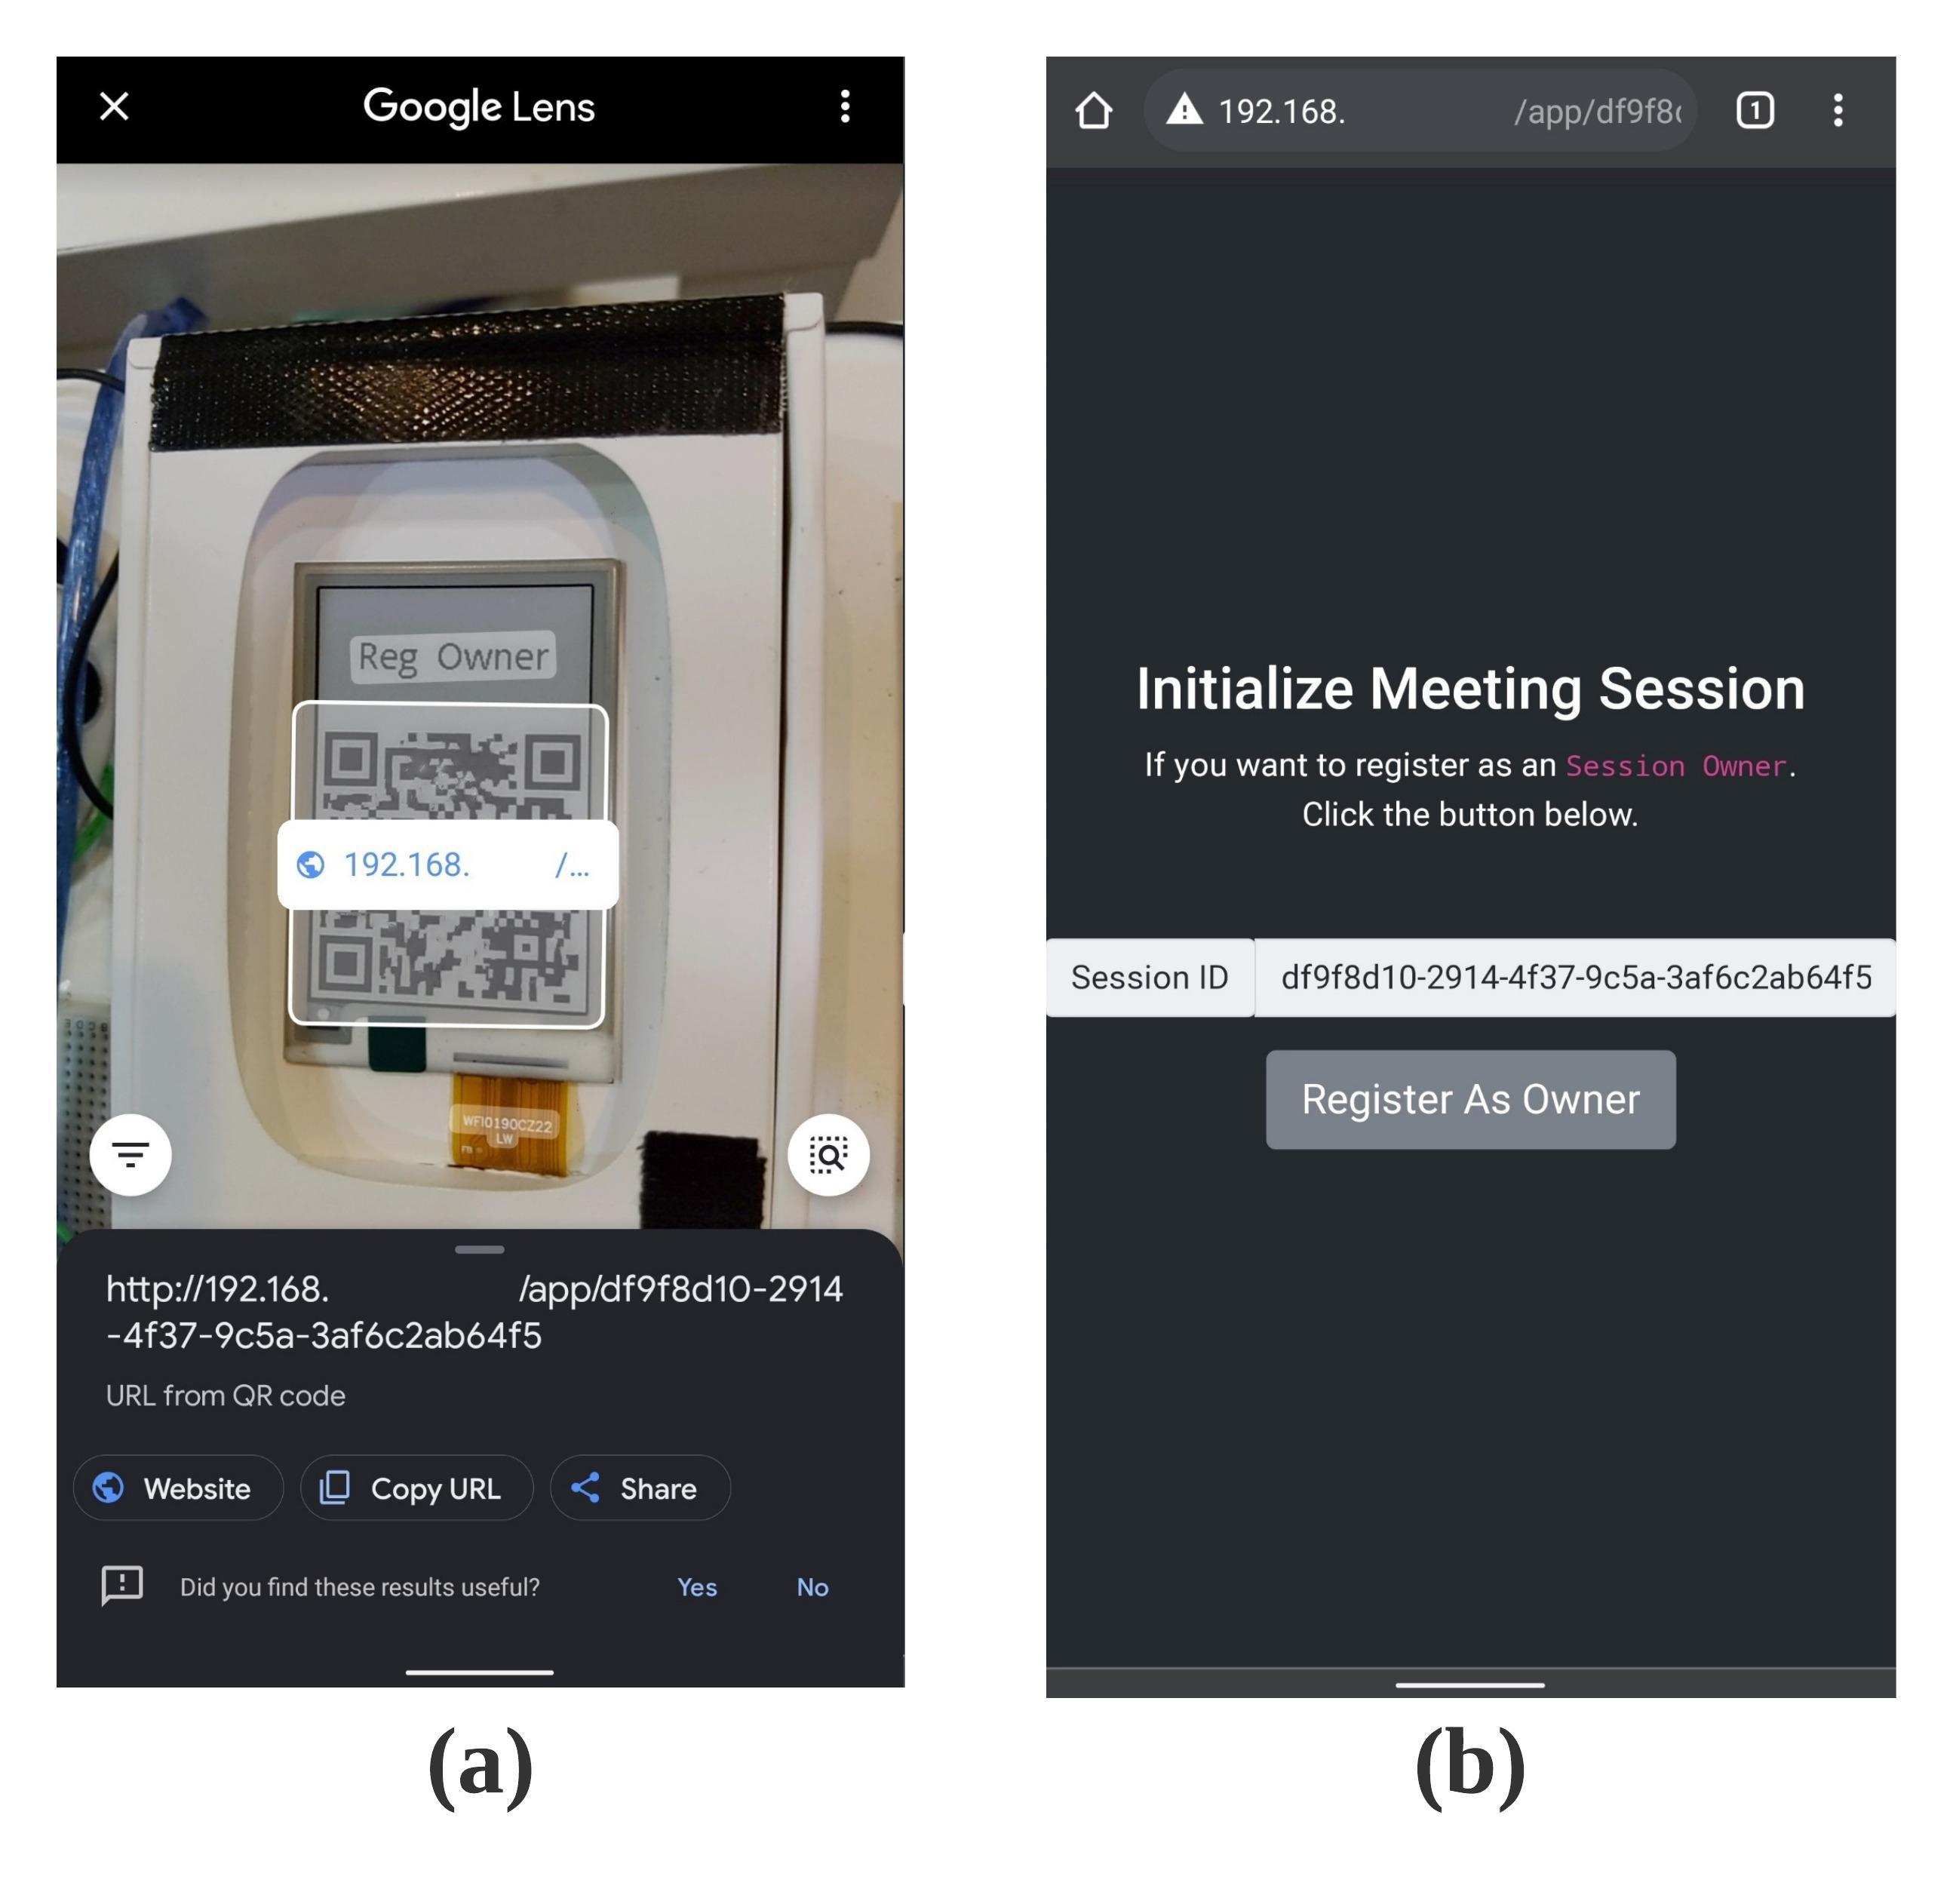
\includegraphics[width=0.6\textwidth]{app-1}
    \caption{行動應用程式會談初始化使用者介面}\label{fig:app-1}
\end{figure}

    在會談對話結束後,會談主持者欲取得當時會談的有效聲音紀錄,須先授權解封伺服器 \DEFserver。
此時會談主持者向解封伺服器 \DEFserver 傳送授權解封聲音會談記錄請求。
如圖 \ref{fig:app-2} \nameref{fig:app-2} (a)。

    解封伺服器 \DEFserver 收到授權解封聲音會談記錄請求後,即依據會談主持者的唯一識別碼 \DEFownerID,
回覆屬於會談主持者的受加密保護的授權金鑰 \DEFakEnc 請會談主持者簽署授權。
如圖 \ref{fig:app-2} \nameref{fig:app-2} (b)。
並透過代表會談主持者身份的私密金鑰,證明會談主持者的身份與授權解封伺服器。
會談主持者的私密金鑰 \DEFprivateKey,透過非對稱式加密演算法之解密函數 \DEFfuncDecSK{},
將受加密保護的授權金鑰 \DEFakEnc 解密,接著使用同一會談主持者的私密金鑰 \DEFprivateKey,
透過數位簽章演算法簽之簽名函數 \DEFfuncSignSK{}。
如圖 \ref{fig:app-2} \nameref{fig:app-2} (c)。

\begin{figure}[H]
    \centering
    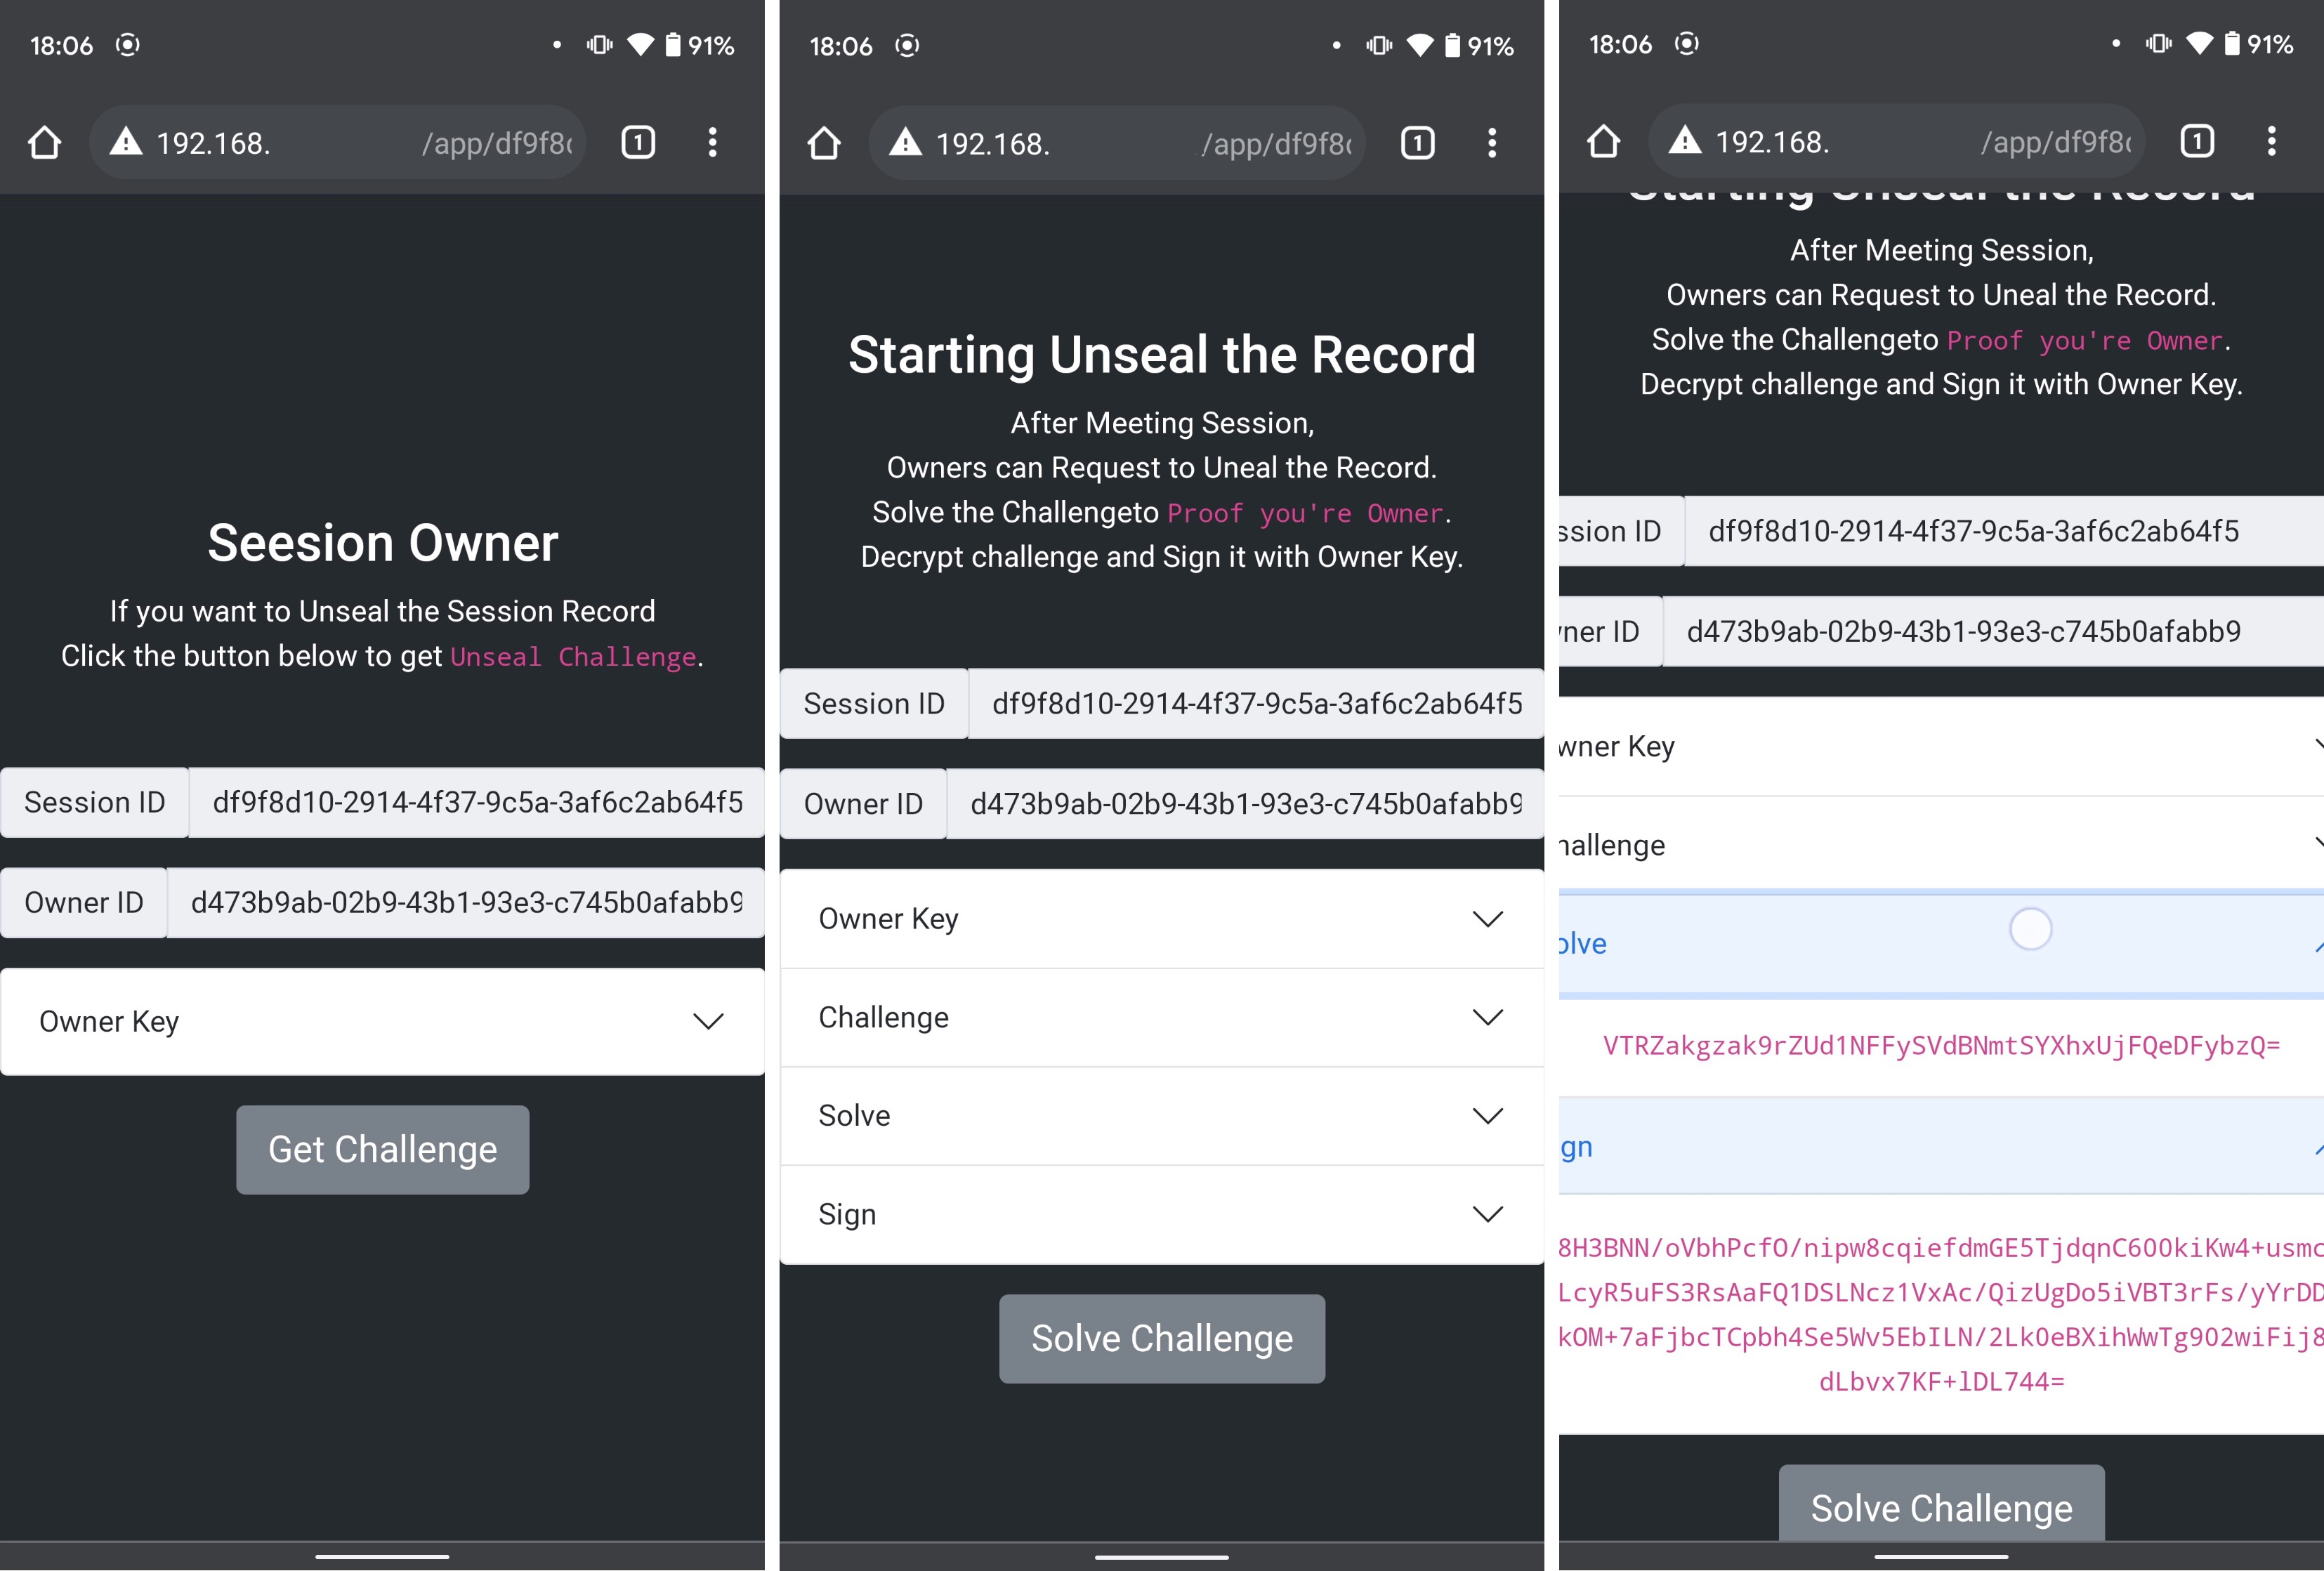
\includegraphics[width=0.9\textwidth]{app-2}
    \caption{行動應用程式會談主持者授權解封伺服器使用者介面}\label{fig:app-2}
\end{figure}

    在會談主持者成功授權解封伺服器 \DEFserver 後,向解封伺服器發起請求取得有效之會談聲音記錄。
如圖 \ref{fig:app-3} \nameref{fig:app-3} (a)。

    此時封伺服器將受加密保護的純噪音之聲音記錄解密,
與含有噪音的受干擾會談聲音記錄透過聲音樣本的離散時間誤差推估函數與自適應噪音消除,還原獲得有效的會談聲音記錄。
執行過程中,如圖 \ref{fig:app-3} \nameref{fig:app-3} (b)。
執行完成後,最終使會談主持者取得此有效之會談聲音記錄。
如圖 \ref{fig:app-3} \nameref{fig:app-3} (c)。

\begin{figure}[H]
    \centering
    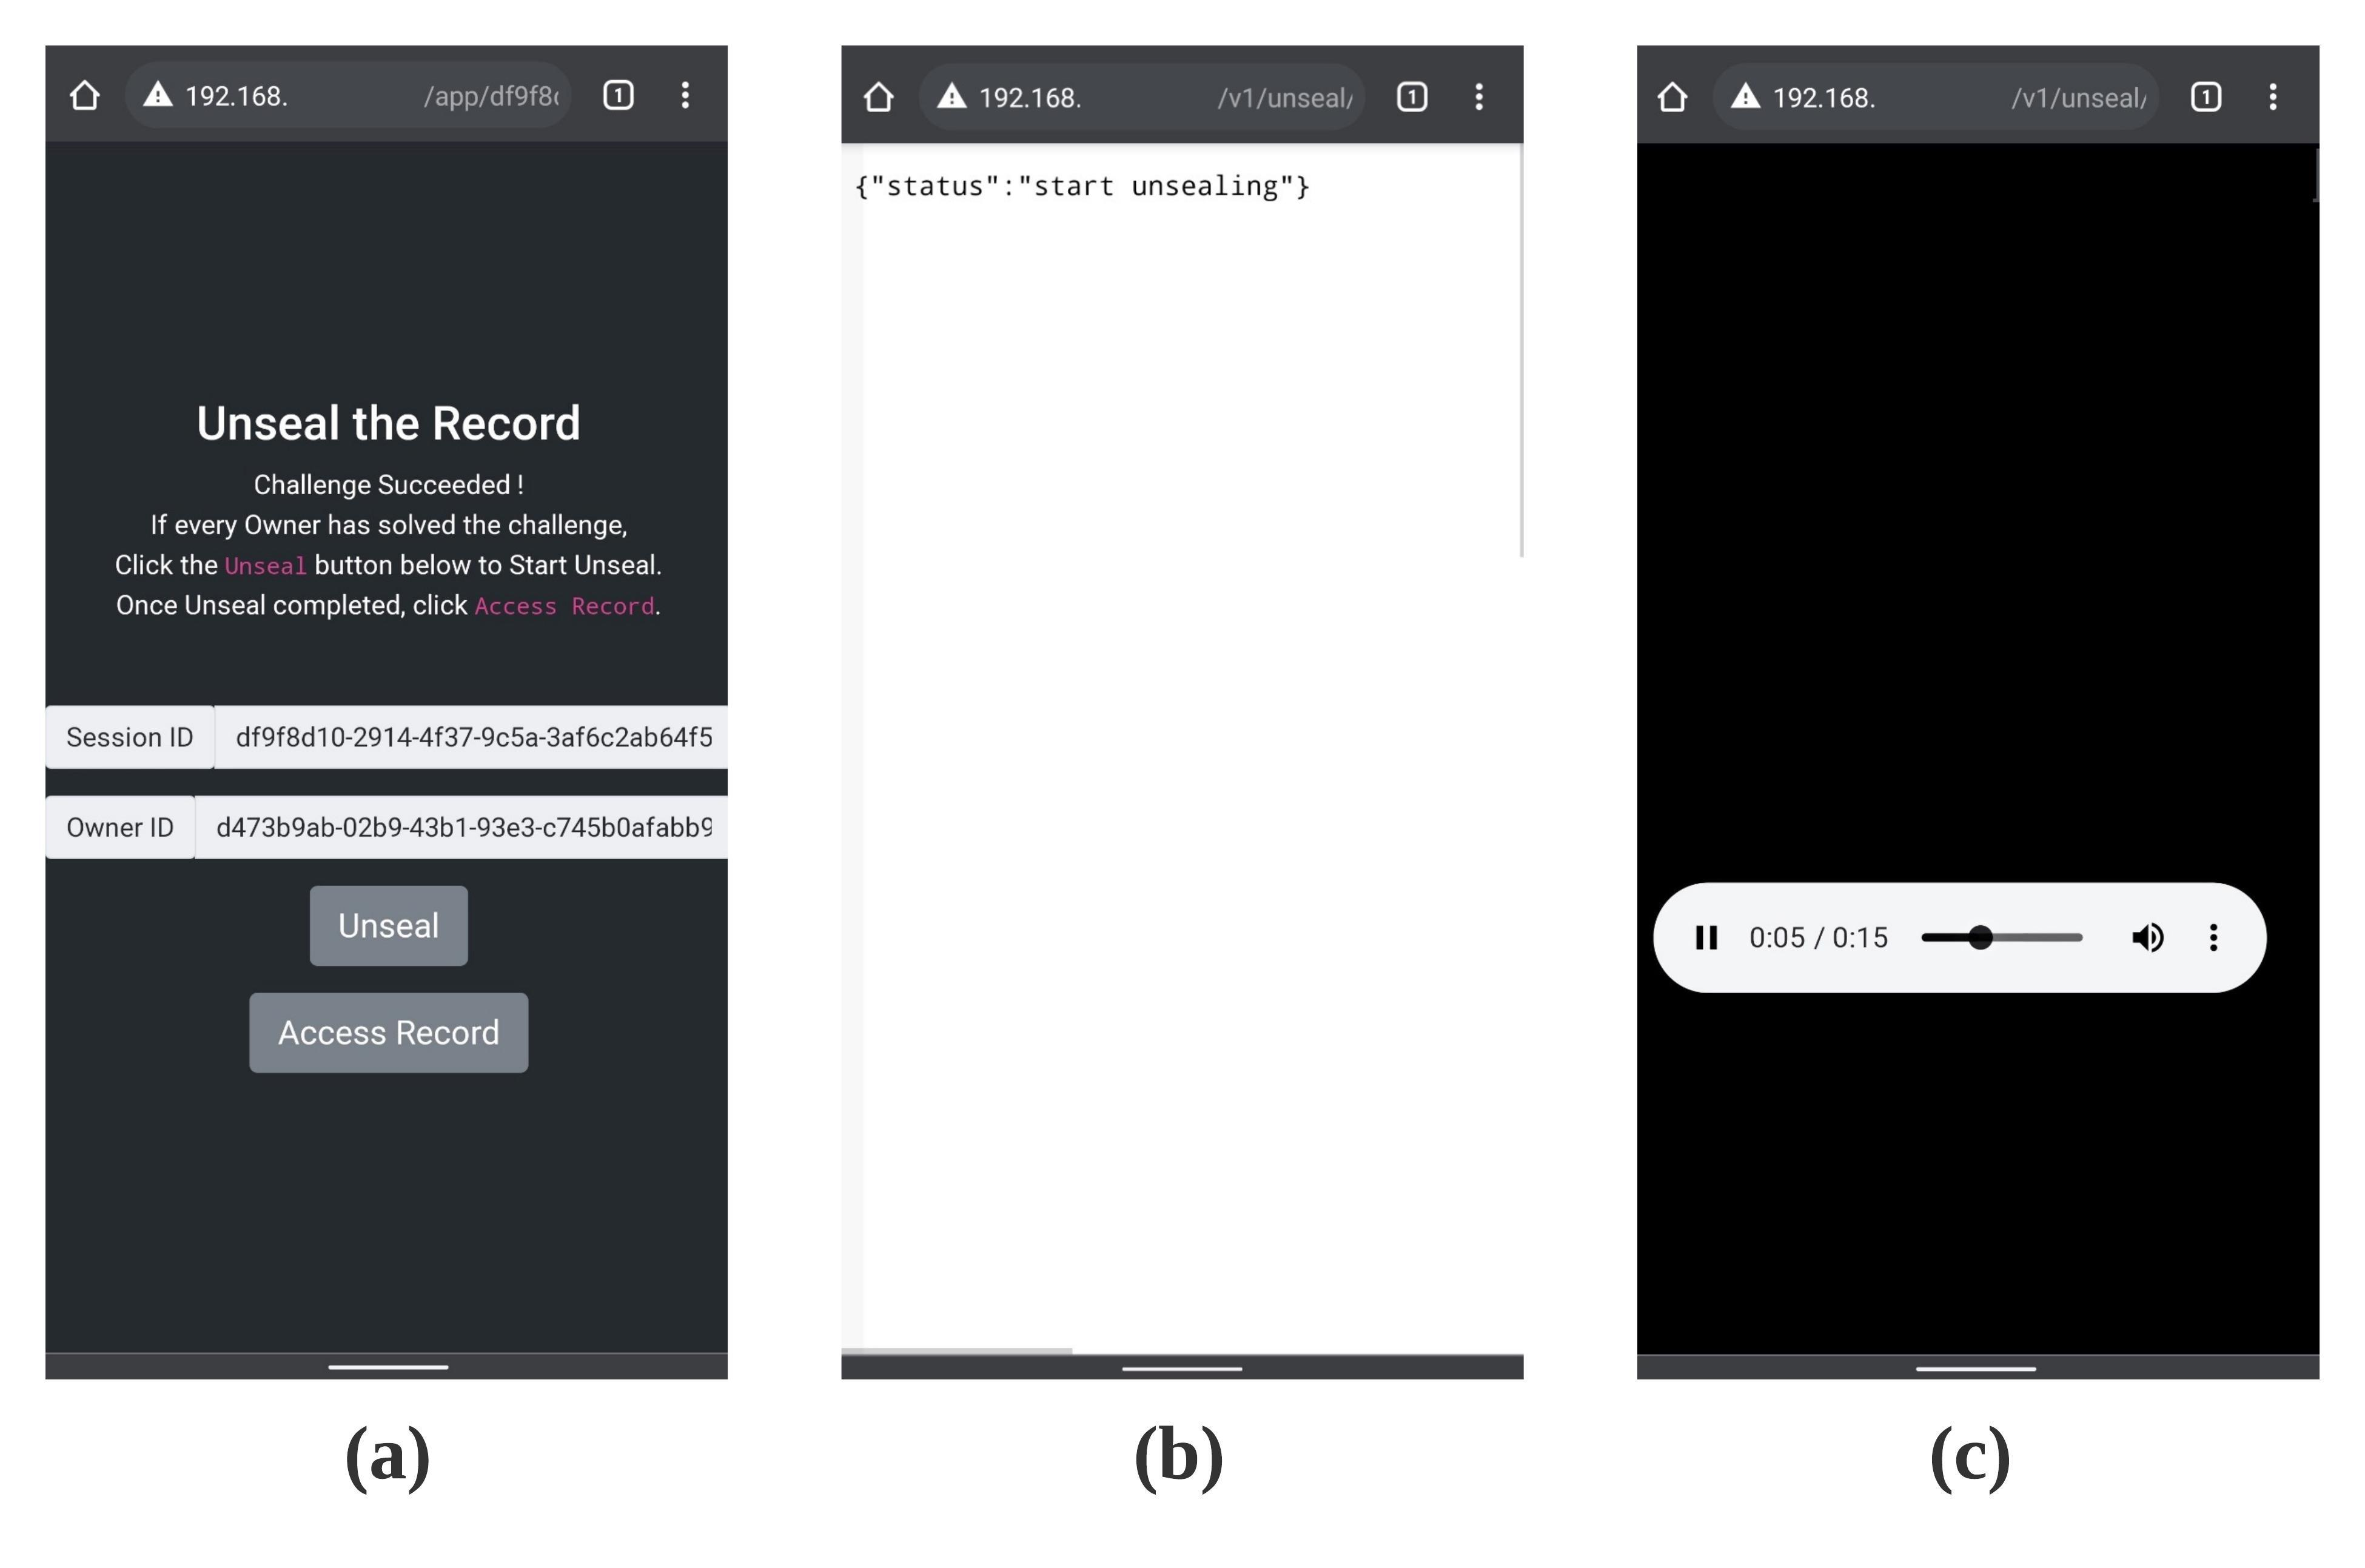
\includegraphics[width=0.9\textwidth]{app-3}
    \caption{行動應用程式取得會談聲音記錄使用者介面}\label{fig:app-3}
\end{figure}


\section{系統實驗}\label{sec:exp}

    本章將透過四個實驗來驗證前篇章節 \ref{sec:impl} \nameref{sec:impl}。
本研究所提出之系統中,當會談結束後本系統會產生兩個聲音紀錄,
分別為超音波麥克風干擾器產生之純噪音聲音紀錄 \DEFrecN,與欲消去噪音的受干擾的會談聲音紀錄 \DEFrecJ。
為得知兩者在不同的信噪比下,超音波麥克風干擾器的干擾效果與主動式噪音消除的效果。
分別設計實驗 \ref{subsec:exp-jammer}、「\nameref{subsec:exp-jammer}」,
與實驗 \ref{subsec:exp-snr-anc}、「\nameref{subsec:exp-snr-anc}」。
接著實驗 \ref{subsec:exp-estm},透過觀察\nameref{subsec:exp-estm}的執行過程,
了解演算法是如何透過最小累計能量差與7個標準差在有效時間內得出對齊點。
最後實驗 \ref{subsec:exp-perform}、「\nameref{subsec:exp-perform}」,
透過輸入的不同時間長度的聲音記錄,來評估分析還原會談聲音記錄的時間複雜度性能。


\subsection{超音波麥克風干擾器之干擾效果分析}\label{subsec:exp-jammer}

    會談終端於會談進行間開啟超音波麥克風干擾器,因此鄰近的麥克風或周邊的聲音記錄裝置,
都將因受到其干擾而失效,場域內的會談參與者無法自行有效記錄會談的聲音內容。
此實驗音目的評估超音波麥克風干擾器產生的干擾噪與音會談聲,
兩者在不同的信噪比下,超音波麥克風干擾器的干擾效果。

    實驗原理為,超音波麥克風干擾器會產生人耳聽不到的干擾聲音。
但是對於麥克風系統卻產生非線性的響應輸出,使超音波投影至人耳可聽見頻譜的聲音,而形成干擾噪音
\cite{chen2019understanding}。
因此透過特別設計的超音波麥克風干擾器,如系統實作\nameref{subsec:impl-mbox},
並調整其輸出干擾聲音的音量,可獲得不同音量的干擾。
本實驗為模擬會談參與者之間的談話內容,使用台灣地區漢語語音噪音下聽辨測試資料集(TMHINT) \cite{wong2007development},
挑選商務會議中可能出現的詞句,並透過 Google 的文字轉換語音服務(TTS)朗讀挑選出詞句文本。
在紀錄受干擾的聲音後評估干擾效果方法為,本實驗使用 Google 所開發的虛擬客觀語音品質估測者(ViSQOL)
\cite{43990}\cite{chinen2020visqol},
為語音品質客觀估測模型 PESQ\cite{rix2001perceptual} 與 POLQA\cite{beerends2013perceptual} 的後繼者。
虛擬客觀語音品質估測者(ViSQOL)根據參考原始聲音(未干擾的會談聲音紀錄)與被干擾的會談聲音紀錄,
透過聲音品質聽感的平均意見分數 MOS-LQO \cite{rec2006p},
從一到五評分客觀語音品質與實際人耳聽感描述,來評估干擾效果。

    實驗儀器使用系統實作 \ref{subsec:impl-mbox} \nameref{subsec:impl-mbox}的超音波麥克風干擾器與錄音克風,
用於產生干擾噪音與錄音。搭配一 IEC 61672-1 標準 Class 2 等級的噪音計 TES-1350A,用於量測聲音分貝值。
實驗環境於背景噪音低於 40 dB的安靜室內空間進行。

    實驗步驟如下,首先於台灣地區漢語語音噪音下聽辨測試資料集(TMHINT)挑選出一標準文本。
接著使用Google 的文字轉換語音(TTS)服務朗讀標準文本,並透過噪音計量測語音朗讀的音量,將朗讀的音量調整至 65 分貝。
接著使用系統實作\nameref{subsec:impl-mbox}的錄音克風,將朗讀標準文本錄音,取得參考原始聲音(未干擾的會談聲音紀律)。
接著透過系統實作\nameref{subsec:impl-mbox}的超音波麥克風干擾器與錄音克風,模擬會談進行時的干擾效果,
並調整干擾器的音量,取得於相同音量的標準文本語音朗讀下,數個不同干擾噪音音量的疊加聲音紀錄。
接著透過聲音紀錄的幅度,計算參考原始聲音(未干擾的會談聲音紀錄)與被干擾的會談聲音紀錄兩者的方均根信噪比。
接著將參考原始聲音(未干擾的會談聲音紀錄)與被干擾的會談聲音紀錄,
透過虛擬客觀語音品質估測者(ViSQOL)得出聲音品質聽感的平均意見分數 MOS-LQO。

    實驗結果如圖 \ref{fig:exp-snr-j} \nameref{fig:exp-snr-j}。$X$ 軸為聲音品質聽感的平均意見分數 MOS-LQO,
$Y$ 軸為參考原始聲音(未干擾的會談聲音紀錄)與被干擾的會談聲音紀錄的信噪比(Signal-to-noise ratio)。
圖 \ref{fig:exp-snr-j} 中,信噪比為零是將參考原始聲音當作被干擾的會談聲音紀錄,即無受干擾的會談聲音紀錄。

\begin{figure}[H]
    \centering
    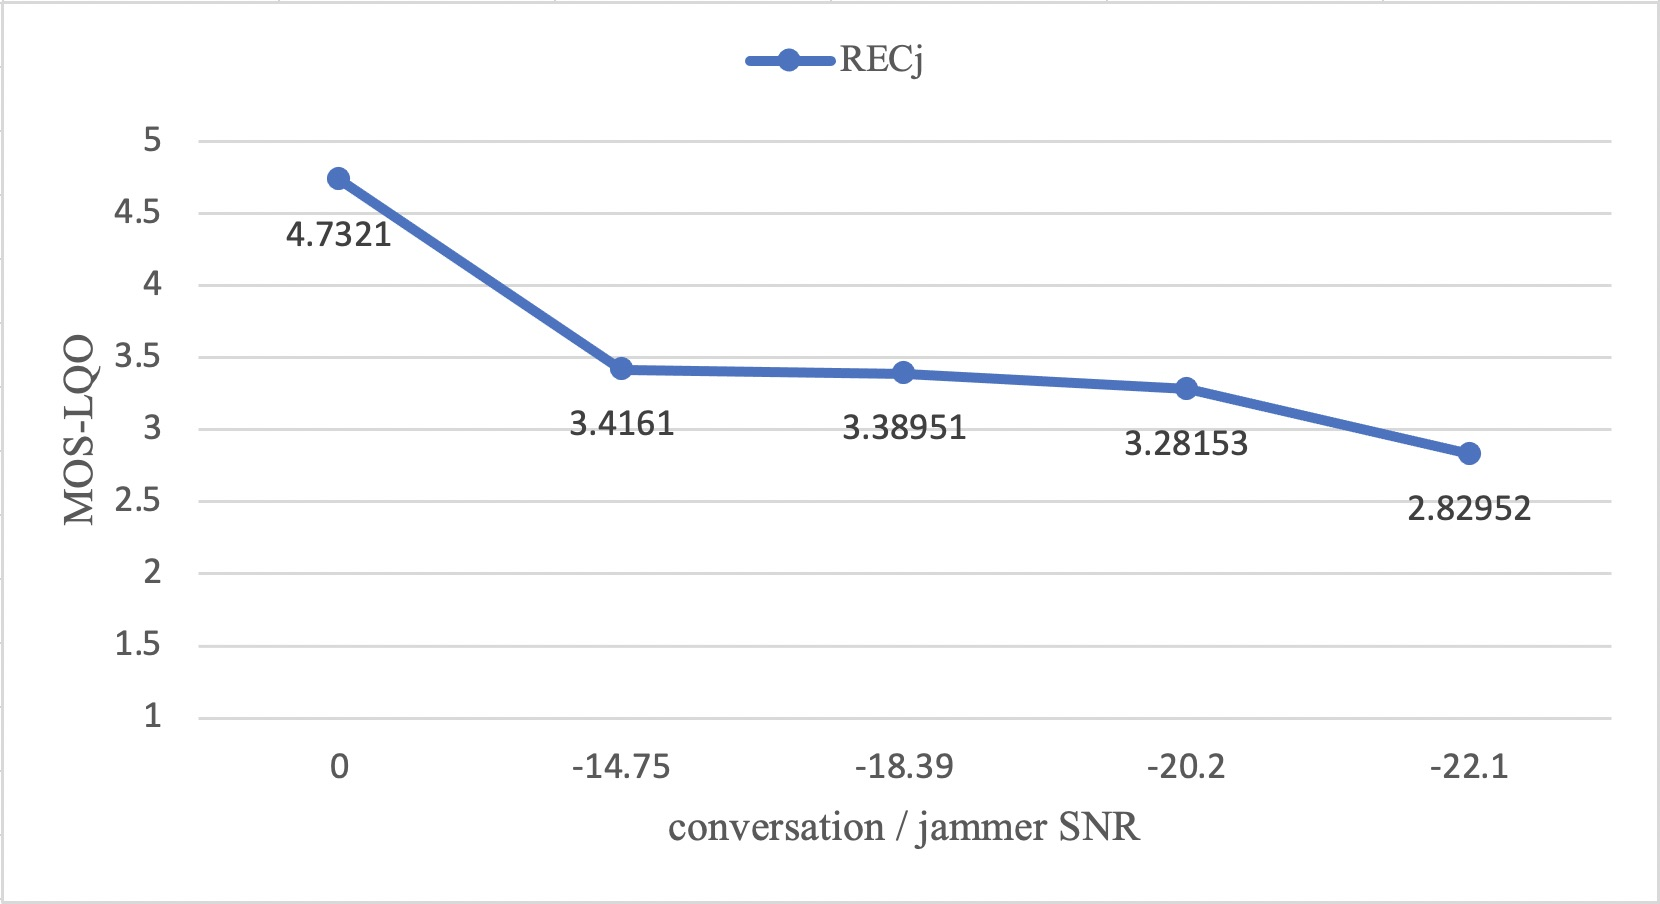
\includegraphics[width=0.8\textwidth]{exp-snr-j}
    \caption{超音波麥克風干擾器之干擾效果}\label{fig:exp-snr-j}
\end{figure}

    觀察實驗結果可以發現,當有開啟麥克風干擾器之後客觀聲音品質聽感平均意見分數 MOS-LQO 顯著下降,
且聲音品質聽感平均意見分數隨著干擾器音量的遞增(SNR遞減)也逐漸降低。
在信噪比達到約 $-22~dB$ 時,聲音品質聽感平均意見分數衰減趨勢增大。
實驗結果對比四種不同信噪比的會談聲音紀錄的客觀聽感描述如下:
隨著干擾器音量的遞增,在信噪比達到約 $-18~dB$ 之前,雖然明顯干擾噪音遞增,但仍免強識別會談對話內容。
信噪比達到約 $-20~dB$ 時,干擾噪音幾乎蓋過會談對話聲音,仍依稀聽有對話聲音,但會談對話內容已無法清楚識別。
當信噪比達到約 $-22~dB$ 時,僅聽得到干擾噪音,無法聽識別出任何其他對話聲音。


\subsection{主動式噪音消除效果分析}\label{subsec:exp-snr-anc}

    當會談主持者欲取得有效的談聲音記錄,除了需要向解封伺服器獲得授權之外,
還需發送請求使解封伺服器執行聲音樣本離散時間推估演算法與主動式噪音消除來還原產生有效的會談聲音紀錄。
此實驗為前篇實驗 \ref{subsec:exp-jammer} \nameref{subsec:exp-jammer} 的延續。
實驗音目的為分析評估超音波麥克風干擾器產生的干擾噪與音會談聲兩者在不同的信噪比下,執行主動式噪音消除的效果。

    實驗原理為,超音波麥克風干擾器產生之純噪音聲音紀錄 \DEFrecN,
與欲消去噪音的受干擾的會談聲音紀錄 \DEFrecJ 中的干擾噪音高度關聯。
因此透過設計一遞移函數,轉換純超音波麥克風干擾器的響應輸出,使其趨近於受干擾的會談聲音紀錄 \DEFrecJ 中的干擾噪音。
透過將受干擾的會談聲音紀錄 \DEFrecJ 中的干擾噪音,減去遞移函數的轉換輸出,完成主動式噪音消除。
此遞移函數為最小均方濾波器(Least Mean Square Filter) \cite{widrow1975adaptive}。

    實驗環境為,
使用系統實作 \ref{subsec:impl-psu} \nameref{subsec:impl-psu} 中的聲音樣本的離散時間誤差推估與自適應噪音消除。
實驗步驟延續前篇實驗 \ref{subsec:exp-jammer} \nameref{subsec:exp-jammer},
但在產生受干擾的會談聲音紀錄時,在同一信噪比的音量設定下,額外產生純噪音聲音紀錄。
接著透過將前篇實驗 \ref{subsec:exp-jammer} \nameref{subsec:exp-jammer} 所產生的受干擾的會談聲音紀錄,
與純噪音聲音紀錄,輸入聲音樣本的離散時間誤差推估與自適應噪音消除,得到還原的會談聲音紀錄。
接著將參考原始聲音(未干擾的會談聲音紀錄)與還原的會談聲音紀錄於不同信造比的組合,
透過虛擬客觀語音品質估測者(ViSQOL)得出聲音品質聽感的平均意見分數 MOS-LQO。

    實驗結果如圖 \ref{fig:exp-snr-rev} \nameref{fig:exp-snr-rev}。$X$ 軸為聲音品質聽感的平均意見分數 MOS-LQO,
$Y$ 軸為參考原始聲音(未干擾的會談聲音紀錄)與被干擾的會談聲音紀錄的信噪比(Signal-to-noise ratio)。

\begin{figure}[H]
    \centering
    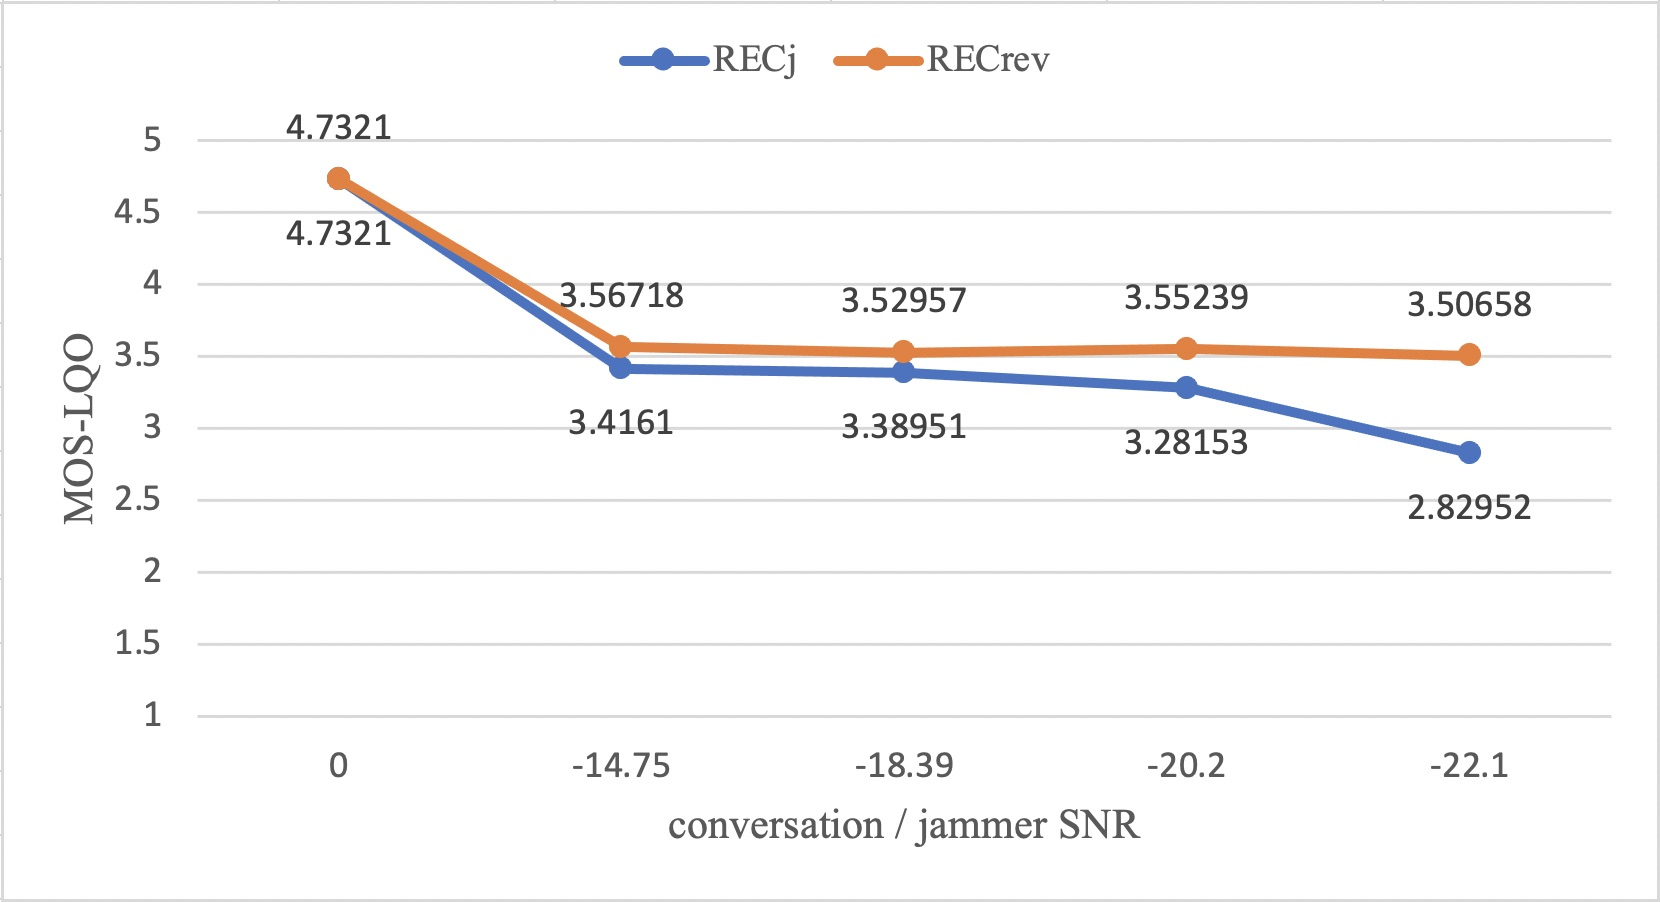
\includegraphics[width=0.8\textwidth]{exp-snr-rev}
    \caption{主動式噪音消除效果}\label{fig:exp-snr-rev}
\end{figure}

    圖 \ref{fig:exp-snr-rev} \nameref{fig:exp-snr-rev}中,
信噪比為零是將參考原始聲音當作被干擾的會談聲音紀錄,即無受干擾的會談聲音紀錄。
圖中藍色折線(\DEFrecJ)為前篇實驗 \ref{subsec:exp-jammer} \nameref{subsec:exp-jammer} 的結果,
為受干擾的會談聲音紀錄的聲音品質聽感的平均意見分數 MOS-LQO。
橘色折線(\DEFrecREV)為執行離散時間誤差推估與自適應噪音消除後,與參考原始聲音(未干擾的會談聲音紀錄)比較,
所得到的聲音品質聽感的平均意見分數 MOS-LQO。

    觀察實驗結果可以發現,在聲音樣本的離散時間誤差推估與自適應噪音消除後,
客觀聲音品質聽感平均意見分數 MOS-LQO 有所提升。
且信噪比達到約 $-22~dB$ 時,雖然受干擾會談聲音紀錄的客觀聲音品質聽感平均意見分數下降明顯(藍色折線\DEFrecJ),
但對於噪音消除後聲音品質聽感平均意見分數的影響不大(橘色折線\DEFrecREV)。
實驗結果對比四種不同信噪比的會談聲音紀錄的客觀聽感描述如下:
隨著干擾器音量的遞增,在信噪比達到約 $-20~dB$ 之前噪音消除後的聲音紀錄皆能清楚識別會談內容。
當信噪比達到約 $-22~dB$ 時,噪音消除前的受干擾會談聲音紀錄僅聽得到干擾噪音,無法聽識別出任何其他對話聲音。
在噪音消除後,還原的聲音紀錄能清楚識別大部分會談內容。


\subsection{聲音樣本離散時間推估演算法}\label{subsec:exp-estm}

    為提升噪音消除的成效,本研究提出聲音樣本離散時間推估演算法
透過將輸入噪音聲音紀錄 \DEFrecN 的離散時間索引值 \DEFpause 加上離散時間誤差值 \DEFshift,
來對齊修正噪音聲音紀錄 \DEFrecN 與欲消去噪音聲音紀錄 \DEFrecJ 的離散時間誤差。
由於純噪音聲音紀錄 \DEFrecN 與受干擾的會談聲音紀錄 \DEFrecJ 中的欲消去噪音,
在時域上波形有著高度關聯性,因此當兩聲音干涉抵銷後的能量會大幅度衰減。
如上所述,本研究提出透過累計整個離散時間序列每個樣本相減(兩聲音干涉抵銷)後總能量差的大小,作為是否對齊的參考指標。

    實驗目的一為觀察離對齊散時間誤差值 \DEFshift 後,兩聲音樣本於離散時間序列上波形對齊。
目的二為觀察動態估計樣本標準差與平均數在執行過程中數值的變化,干涉抵銷後總能量差為最小值,
且評估演算法終止條件是否符合預期,以解決歷遍所有可能總能量差的時間複雜度膨脹快速問題。
原理如 \ref{subsec:exp-jammer} \nameref{subsec:exp-jammer}所述。

    實驗環境為兩聲音樣本,包含純噪音聲音紀錄 \DEFrecN,與欲消去噪音的會談聲音紀錄 \DEFrecJ。
實驗步驟如下:首先觀察兩樣本於離散時間上波形的前後誤差;接著執行此演算法得知離散時間誤差值 \DEFshift,
並實時輸出聲音樣本離散時間推估演算法執行時本標準差與平均數的數值並記錄;
接著觀察離散時間索引值 \DEFpause 加上離散時間誤差值 \DEFshift 後兩樣本於離散時間上波形的前後誤差;
最後分析各項數值於執行過程中數值的變化。此實驗聲音樣本以取樣率 \DEFsamplerate $= 44100$ 為例。

    實驗結果如下。
如圖 \ref{fig:exp-shift-1} 為兩聲音樣本包含純噪音聲音紀錄 \DEFrecN,
與欲消去噪音的會談聲音紀錄 \DEFrecJ,在會談結束後尚未執行齊前,於離散時間上波形的前後誤差。
圖為擷取取時間長度 1.2 秒,共長約52920 ($44100 \times 1.2 $) 個樣本。
可以觀察到兩相似波形,於離散時間上誤差約 1800 個樣本週期。

\begin{figure}[H]
    \centering
    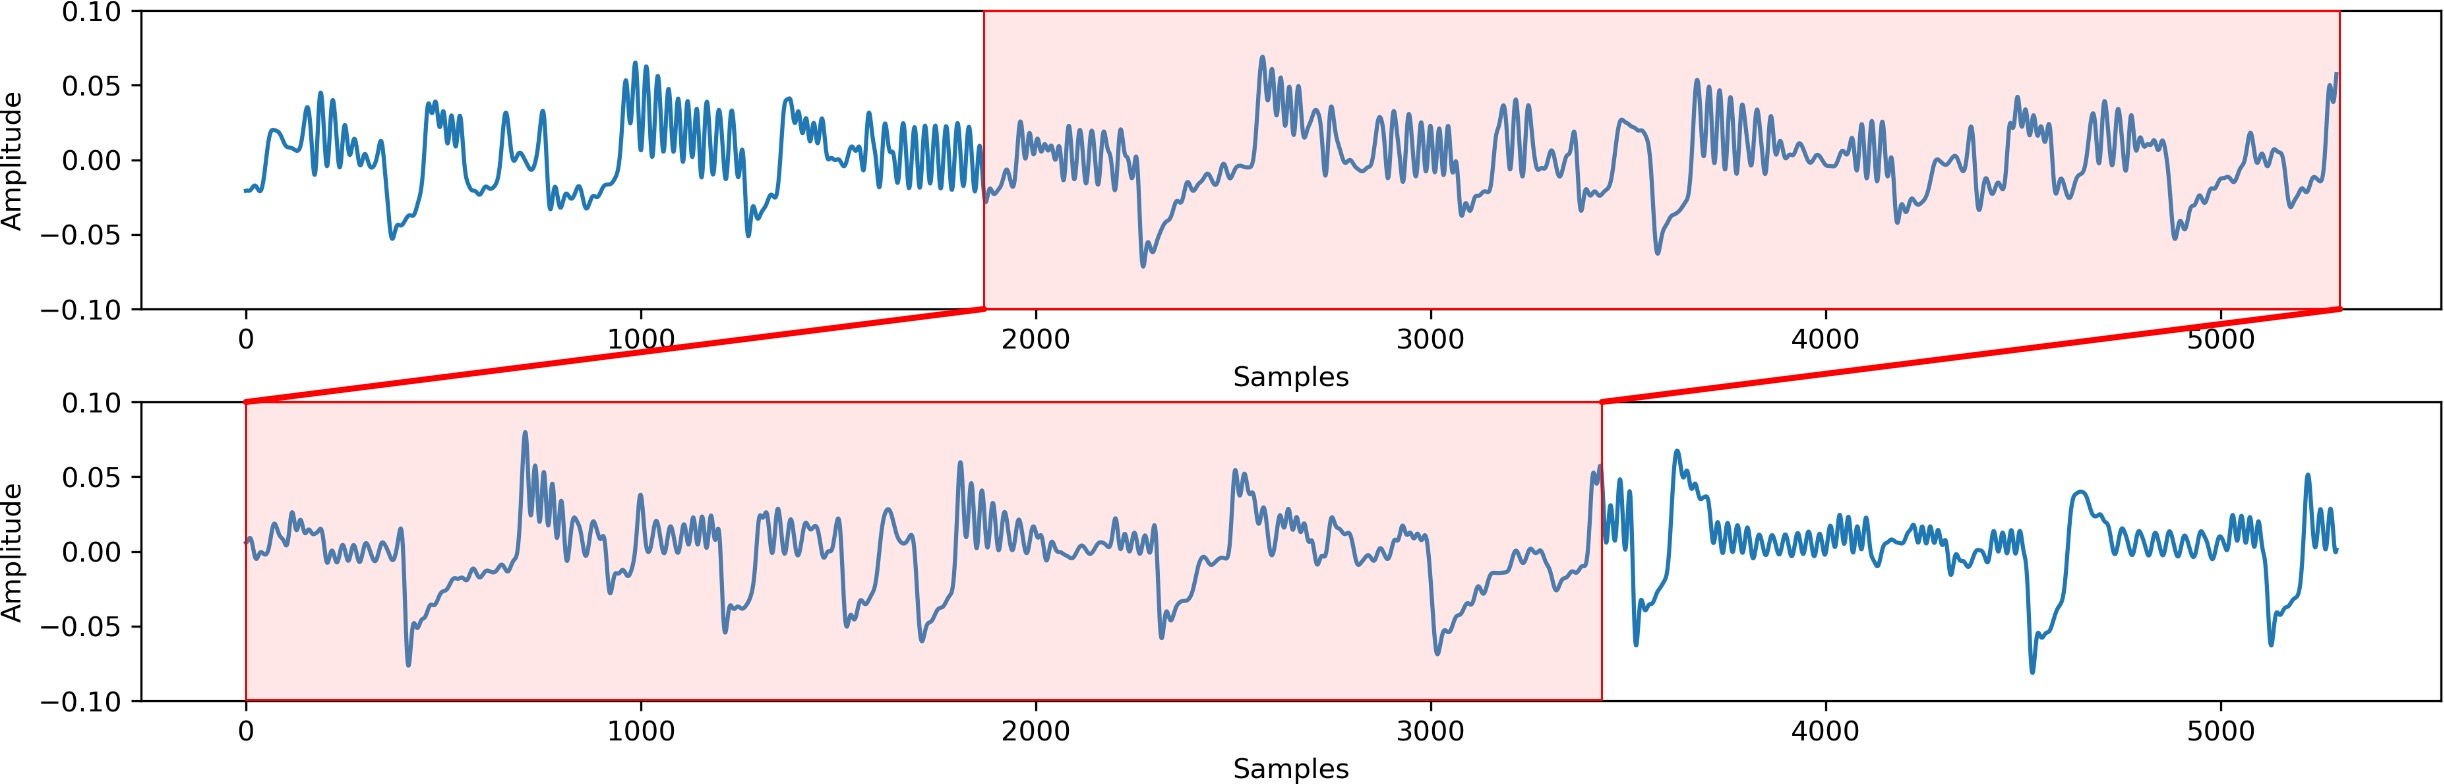
\includegraphics[width=0.9\textwidth]{exp-shift-1}
    \caption{聲音樣本對齊前波形圖}\label{fig:exp-shift-1}
\end{figure}

    \nameref{fig:exp-shift-2}如 \ref{fig:exp-shift-2},當兩聲音樣本純噪音聲音紀錄 \DEFrecN
與欲消去噪音的會談聲音紀錄 \DEFrecJ,在執行聲音樣本離散時間推估演算法得知離散時間誤差值 \DEFshift 後。
將純噪音聲音紀錄 \DEFrecN 的離散時間序列索引值 \DEFpause 加上離散時間誤差值 \DEFshift
來修正兩聲音樣本的離散時間誤差。
此實驗為例,執行所得到離散時間誤差值 \DEFshift $=1866$,即離散時間序列上,
純噪音聲音紀錄 \DEFrecN 平移 $1866$ 個樣本週期來修正兩聲音樣本的離散時間誤差。
圖為擷取取時間長度 1.2 秒,共長約52920 ($44100 \times 1.2 $) 個樣本。
可以觀察到兩相似波形,於離散時間已經達到單位取樣週期等級的對齊。

\begin{figure}[H]
    \centering
    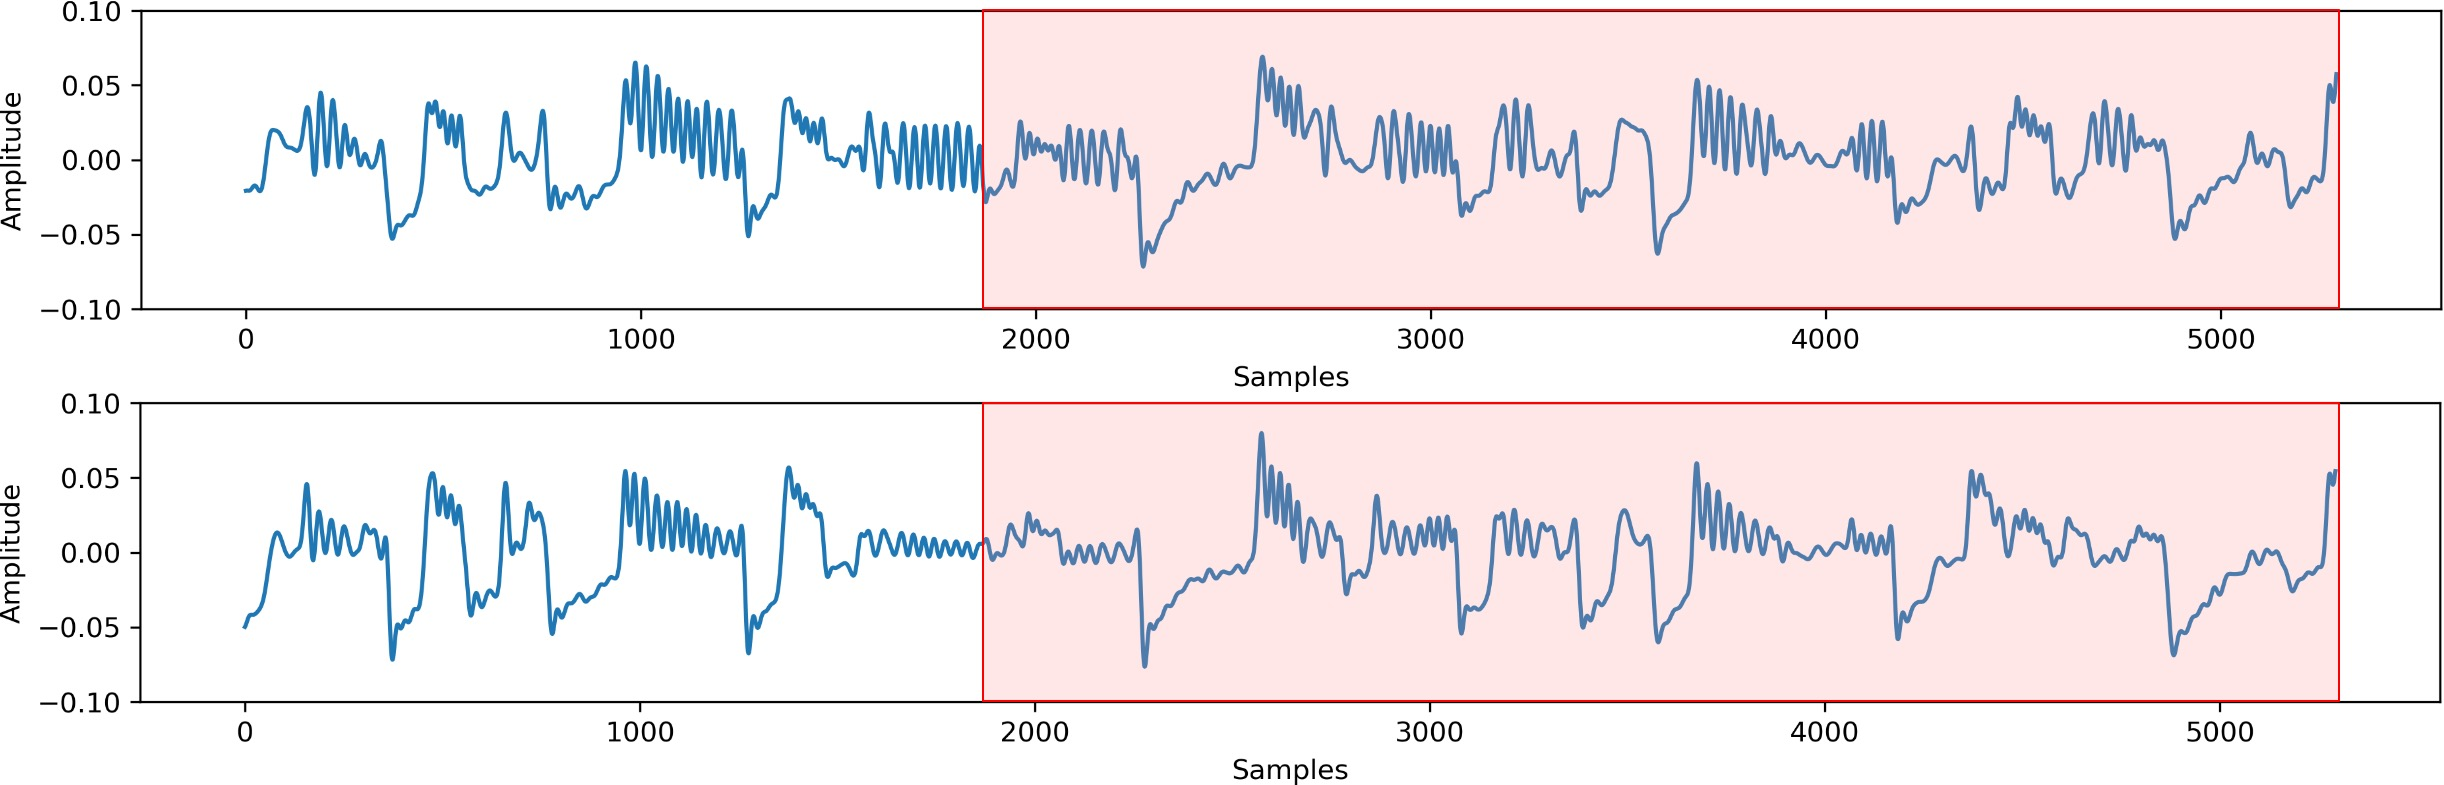
\includegraphics[width=0.9\textwidth]{exp-shift-2}
    \caption{聲音樣本對齊後波形圖}\label{fig:exp-shift-2}
\end{figure}

    聲音樣本離散時間推估演算法執行時數值如圖 \ref{fig:exp-shift-3}。
包含干涉抵銷後之總能量差(紅);目前最小的干涉抵銷後之總能量差(紅);
干涉抵銷後之總能量差的樣本標準差(藍);干涉抵銷後之總能量差的平均(綠);
$X$ 軸為總能量差的幅值大小,正比於能量的平方根,$Y$ 軸為動態相對平移量 \DEFcandiSFT。

\begin{figure}[H]
    \centering
    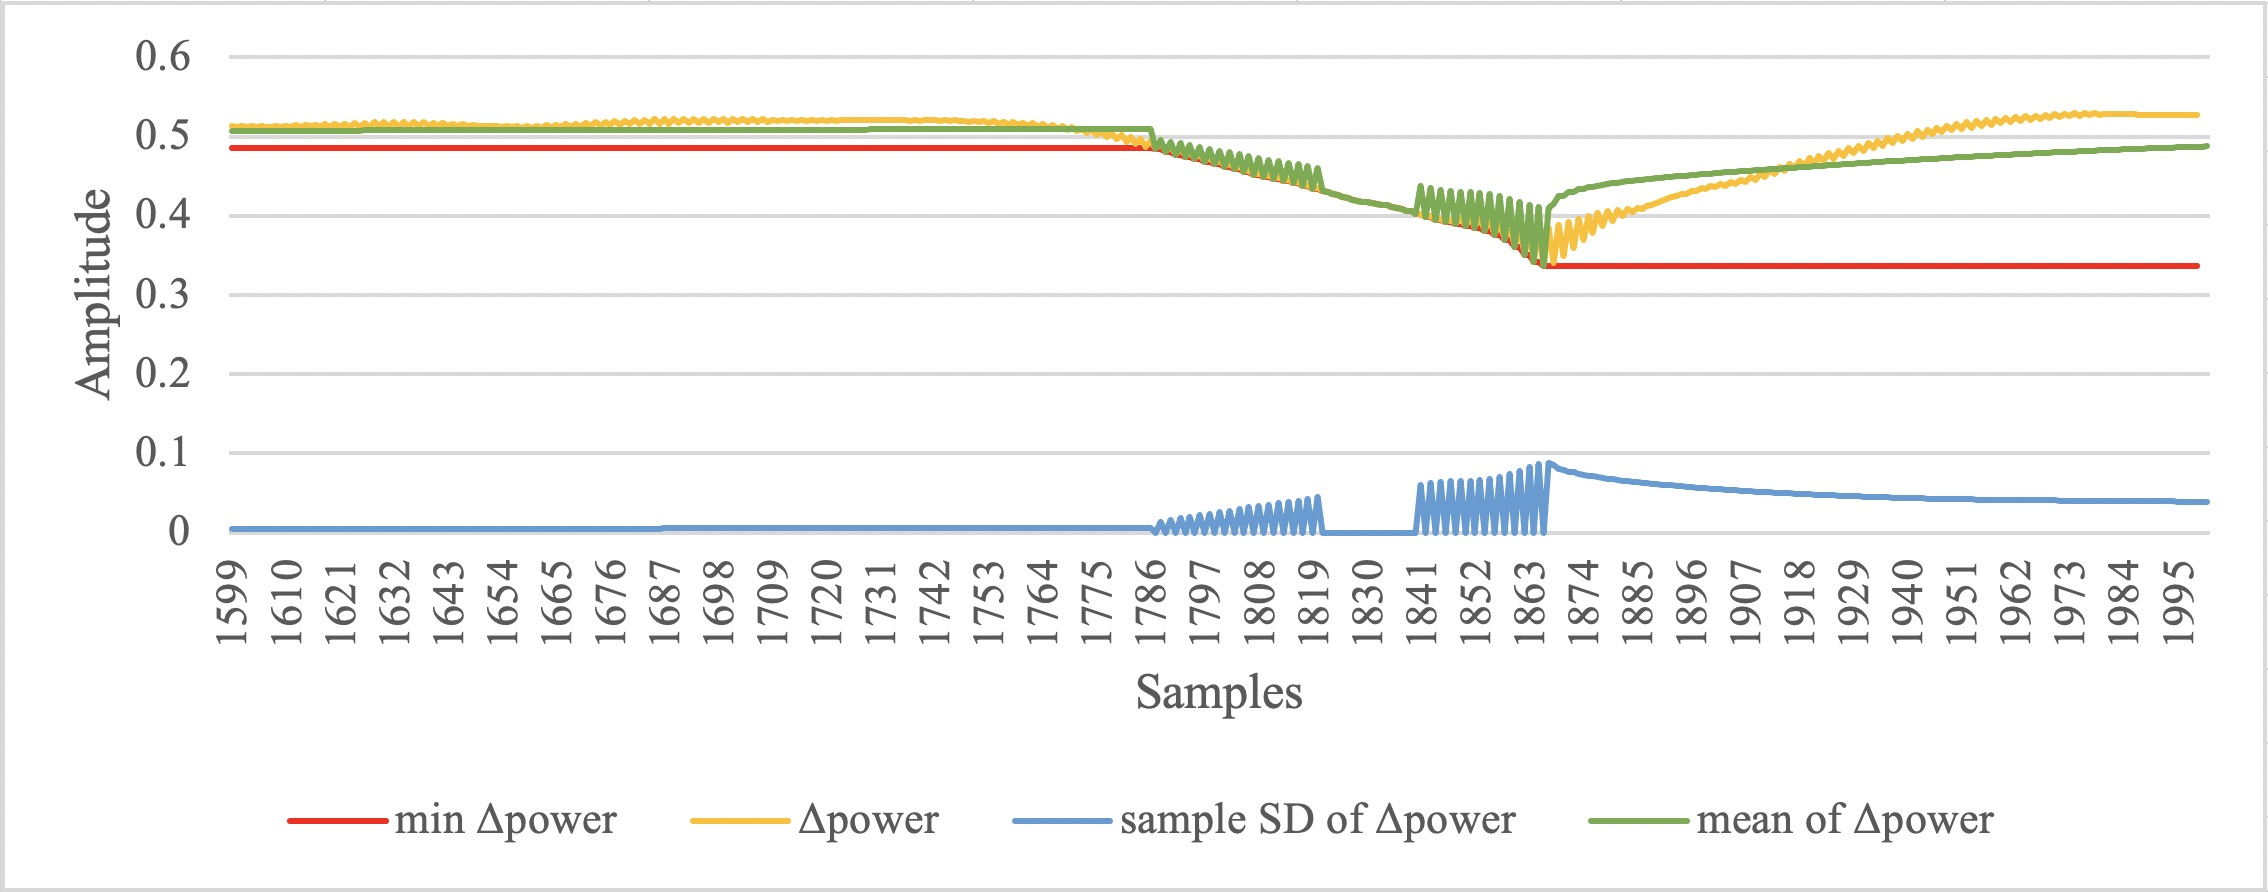
\includegraphics[width=0.85\textwidth]{exp-shift-3}
    \caption{聲音樣本離散時間推估演算法執行時數值變化圖}\label{fig:exp-shift-3}
\end{figure}

    聲音樣本離散時間推估演算法執行時,於每次迭代中動態估計樣本標準差與平均數。
並且於每次找到新的最小總能量差時,將樣本標準差賦值為$0$,平均數賦值為此最小總能量差。
圖中可以觀察到每次目前最小總能量差更新時,平均數會在最小總能量差與理論整體平均之間震盪,
樣本標準差則會在$0$與理想母體標準差之間震盪,如圖 \ref{fig:exp-shift-3}。

    為找到有效找到最小總能量差,本研究透過七倍標準差(藍),來判斷目前最小總能量差來判斷是否為全域最小總能量差。
其中最小累積能量差與七倍標準差於執行過程中數值變化如圖 \ref{fig:exp-shift-4}。

\begin{figure}[H]
    \centering
    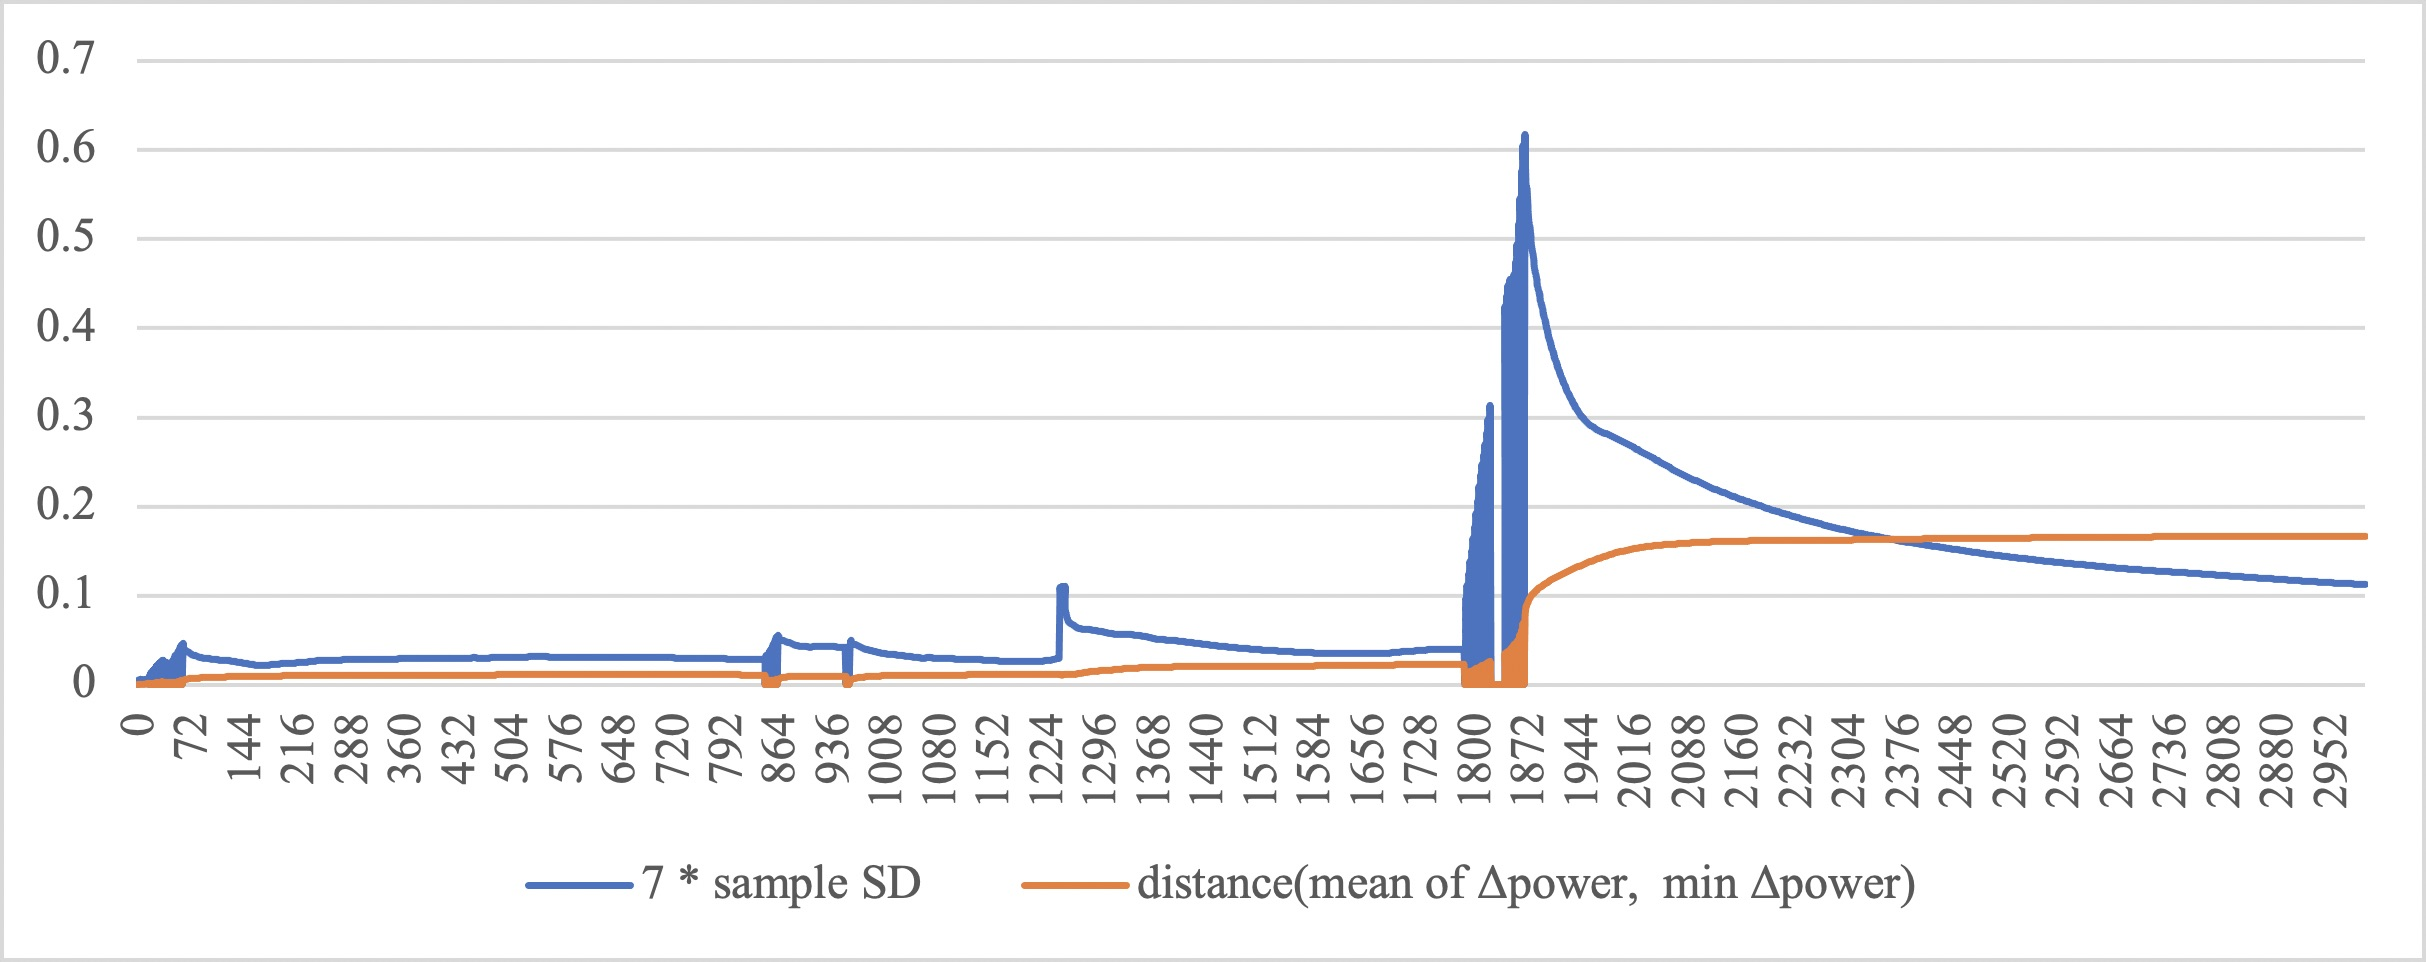
\includegraphics[width=0.85\textwidth]{exp-shift-4}
    \caption{最小累積能量差與七倍標準差數值變化圖}\label{fig:exp-shift-4}
\end{figure}

    如圖 \ref{fig:exp-shift-4} 聲音樣本離散時間推估演算法執行過程中會持續更新目前最小總能量差,
透過計算目前最小總能量差與總能量差的平均的距離(橘),可以得知目前最小總能量位於多少標準差的區間。
若新很長的時間都未更新最小總能量差時,此時平均數會逐漸趨近理論整體平均,樣本標準差也逐漸趨近母體標準差。
當目前最小總能量差與平均距離超過七倍樣本標準差(藍與橘交叉)時,則認定目前最小總能量差為全域最小總能量差。
而計算出目前最小總能量差時的動態相對平移量 \DEFcandiSFT,則為認定聲音樣本的離散時間誤差 \DEFshift。

    此實驗為例,執行所得到離散時間誤差值 \DEFshift $=1866$,如圖 \ref{fig:exp-shift-3},
在平移量 \DEFcandiSFT $=1866$ 時,得到目前最小總能量差。
而在平移量 \DEFcandiSFT $=2376$ 時,目前最小總能量差與平均距離超過七倍樣本標準差(藍與橘交叉),
則演算法終止,完成此聲音樣本離散時間推估演算法。


\subsection{還原會談聲音記錄性能分析}\label{subsec:exp-perform}

    當會談主持者欲取得有效的談聲音記錄,除了需要向解封伺服器獲得授權之外,
還需發送請求使解封伺服器執行聲音樣本離散時間推估演算法與主動式噪音消除來還原產生有效的會談聲音紀錄。
此實驗目的為評估分析當還原會談聲音記錄時,封伺服器執行聲音樣本離散時間推估演算法與主動式噪音消除的時間複雜度性能為何。
實驗原理為透過膨脹輸入的聲音記錄時間長度,來評估分析還原會談聲音記錄的時間複雜度性能。
透過會談內容相似,但時間長度 \DEFtimeREC 不同的受干擾會談聲音記錄 \DEFrecJ,
執行聲音樣本離散時間推估演算法 \DEFfuncEstm{} 與主動式噪音消除 \DEFfuncAnc{},可以得到不同的執行時間。
透過分析執行時間與聲音記錄時間長度的變化,得知其時間複雜度性能。

    實驗環境為透過系統實作 \ref{subsec:impl-mbox} \nameref{subsec:impl-mbox}的超音波麥克風干擾器與錄音克風,
產生數個不同時間長度的干擾純噪音 \DEFrecN 與會談錄音 \DEFrecJ。
於相同算力的計算資源平台上,執行聲音樣本離散時間推估演算法 \DEFfuncEstm{} 與主動式噪音消除 \DEFfuncAnc{},
本實驗算力平台以 AMD R5 4650GE 為例(Passmark指標約16000分)為例。
並在執行各階段加入時間戳記,於執行完成分析時計算時間戳記的差,得出執行時間。

    實驗步驟如下:首先模擬會談的進行,會談內容為相似聲音(重複朗讀相同的文本),
會談進行時開啟超音波麥克風干擾器,透過麥克風紀錄此受干擾會談聲音記錄。
在另外產生相同時間長度的純噪音 \DEFrecN。
透過重複上述步驟,並控制聲音紀錄的時間於數個不同的長度。
最後於計算資源平台上,執行聲音樣本離散時間推估演算法 \DEFfuncEstm{} 與主動式噪音消除 \DEFfuncAnc{},
求得不同聲音記錄時間長度下,不同的執行時間。
聲音紀錄時間長度 \DEFtimeREC 共有九種,最短從15秒至最長1小時,聲音紀錄時間長度的步進以指數成長 2 倍為原則。
聲音樣本離散時間推估演算法 \DEFfuncEstm{} 與主動式噪音消除 \DEFfuncAnc{},兩者接續執行,執行時間互不重疊。
並計算兩者時間加總為總實行時間。

    實驗結果如表 \ref{table:exp-time} 與圖 \ref{fig:exp-time}。
透過觀察實驗結果可已得知,聲音樣本離散時間推估演算法與主動式噪音消除,時間複雜度皆趨近於線性 $O(n)$。
兩者的執行時間加總,時間複雜度表現也同樣趨近於線性 $O(n)$。

\begin{longtable}{| r | c | c | c |}
    \caption{還原會談聲音記錄執行時間表}\label{table:exp-time} \\
    \hline
    \multicolumn{1}{|r|}{錄音長度} &
    \multicolumn{1}{|c|}{\DEFfuncEstm{} 執行時間} &
    \multicolumn{1}{|c|}{\DEFfuncAnc{} 執行時間} &
    \multicolumn{1}{|c|}{總執行時間 (秒)} \\
    \hline
    \endfirsthead

    \multicolumn{1}{|r|}{錄音長度} &
    \multicolumn{1}{|c|}{\DEFfuncEstm{} 執行時間} &
    \multicolumn{1}{|c|}{\DEFfuncAnc{} 執行時間} &
    \multicolumn{1}{|c|}{總執行時間 (秒)} \\
    \hline
    \endhead

    \hline
    \endlastfoot

    15 秒 & 3.67秒 & 12.63秒 & 16.3秒 \\

    30 秒 & 7.23 秒 & 24.38 秒 & 31.61 秒 \\

    1 分鐘 & 14.35 秒 & 47.51 秒 & 61.86 秒 \\

    3 分鐘 & 28.5 秒 & 93.77 秒 & 122.27 秒 \\

    5 分鐘 & 71.72 秒 & 234.7 秒 & 306.42 秒 \\

    10 分鐘 & 141.98 秒 & 471.61 秒 & 613.6 秒 \\

    20 分鐘 & 279.96 秒 & 929.56 秒 & 1209.52 秒 \\

    30 分鐘 & 356.37 秒 & 1389.75 秒 & 1746.12 秒 \\

    1小 時 & 528.22 秒 & 2765.89 秒 & 3294.11 秒 \\
\end{longtable}

    圖 \ref{fig:exp-time} 為表 \ref{table:exp-time} 中資料所繪製,
$Y$軸為聲音紀錄時間長度 \DEFtimeREC,$X$軸為執行時間。
圖中將聲音樣本離散時間推估演算法 \DEFfuncEstm{} (綠色菱形點線Estm)、
主動式噪音消除 \DEFfuncAnc{}(藍色方形點線ANC)與兩者時間加總(黃色三角形點線Total),分別繪制於三條折線。

\begin{figure}[H]
    \centering
    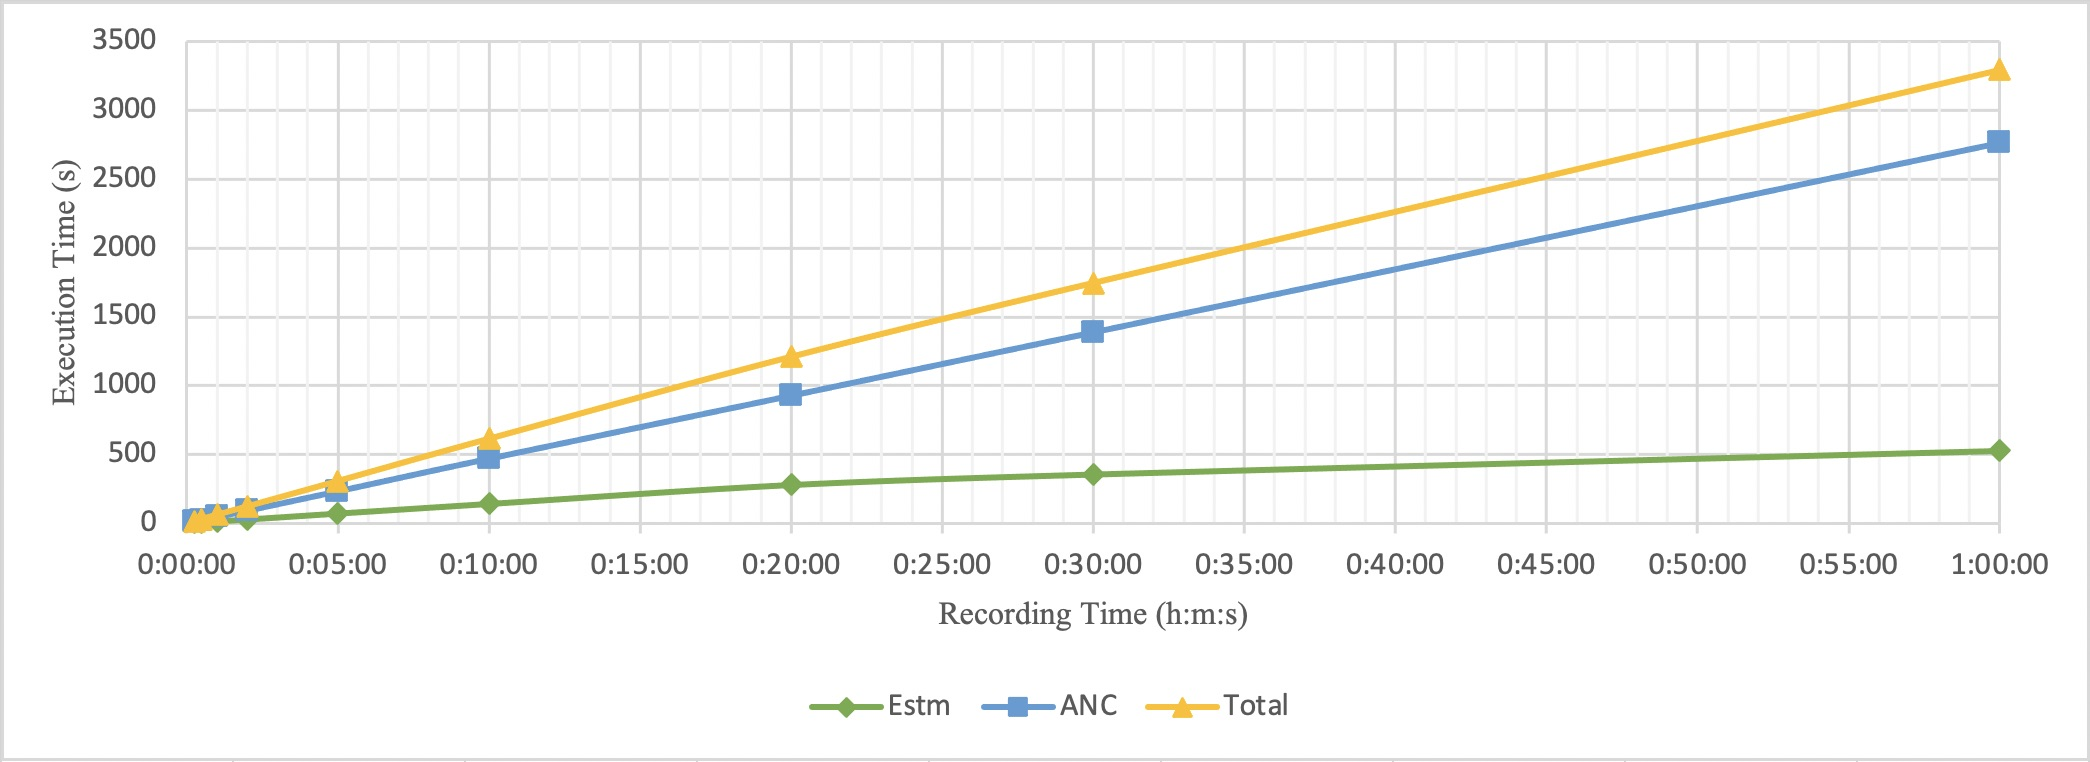
\includegraphics[width=0.85\textwidth]{exp-time}
    \caption{還原會談聲音記錄執行時間圖}\label{fig:exp-time}
\end{figure}


\section{系統安全性分析}\label{sec:analysis}

    此章節將針對本研究所設計之系統分為兩部分進行安全性的探討,
一、「超音波麥克風干擾器與主動式噪音控制」;二、「聲音記錄存取控制協定」;


\subsection{超音波麥克風干擾器與主動式噪音控制}

    概覽本研究所設計之\nameref{fig:system-data-flow},如圖 \ref{fig:system-data-flow}。
透過圖中上半部分可以觀察到,系統透過超音波麥克風干擾器(Jammer),將會談參與者(Attender)的對話內容加以保密,
產生受干擾的會談聲音記錄 \DEFrecJ。並透過同一超音波麥克風干擾器,產生用於降噪還原的純噪音之聲音記錄 \DEFrecN。
最後經過 \DEFfuncEstm{} 與 \DEFfuncAnc{} 降噪還原出 \DEFrecREV。
接續段落將此超音波麥克風干擾器與主動式噪音控制視為一串流加密系統進行安全性分析。

\begin{figure}[H]
    \centering
    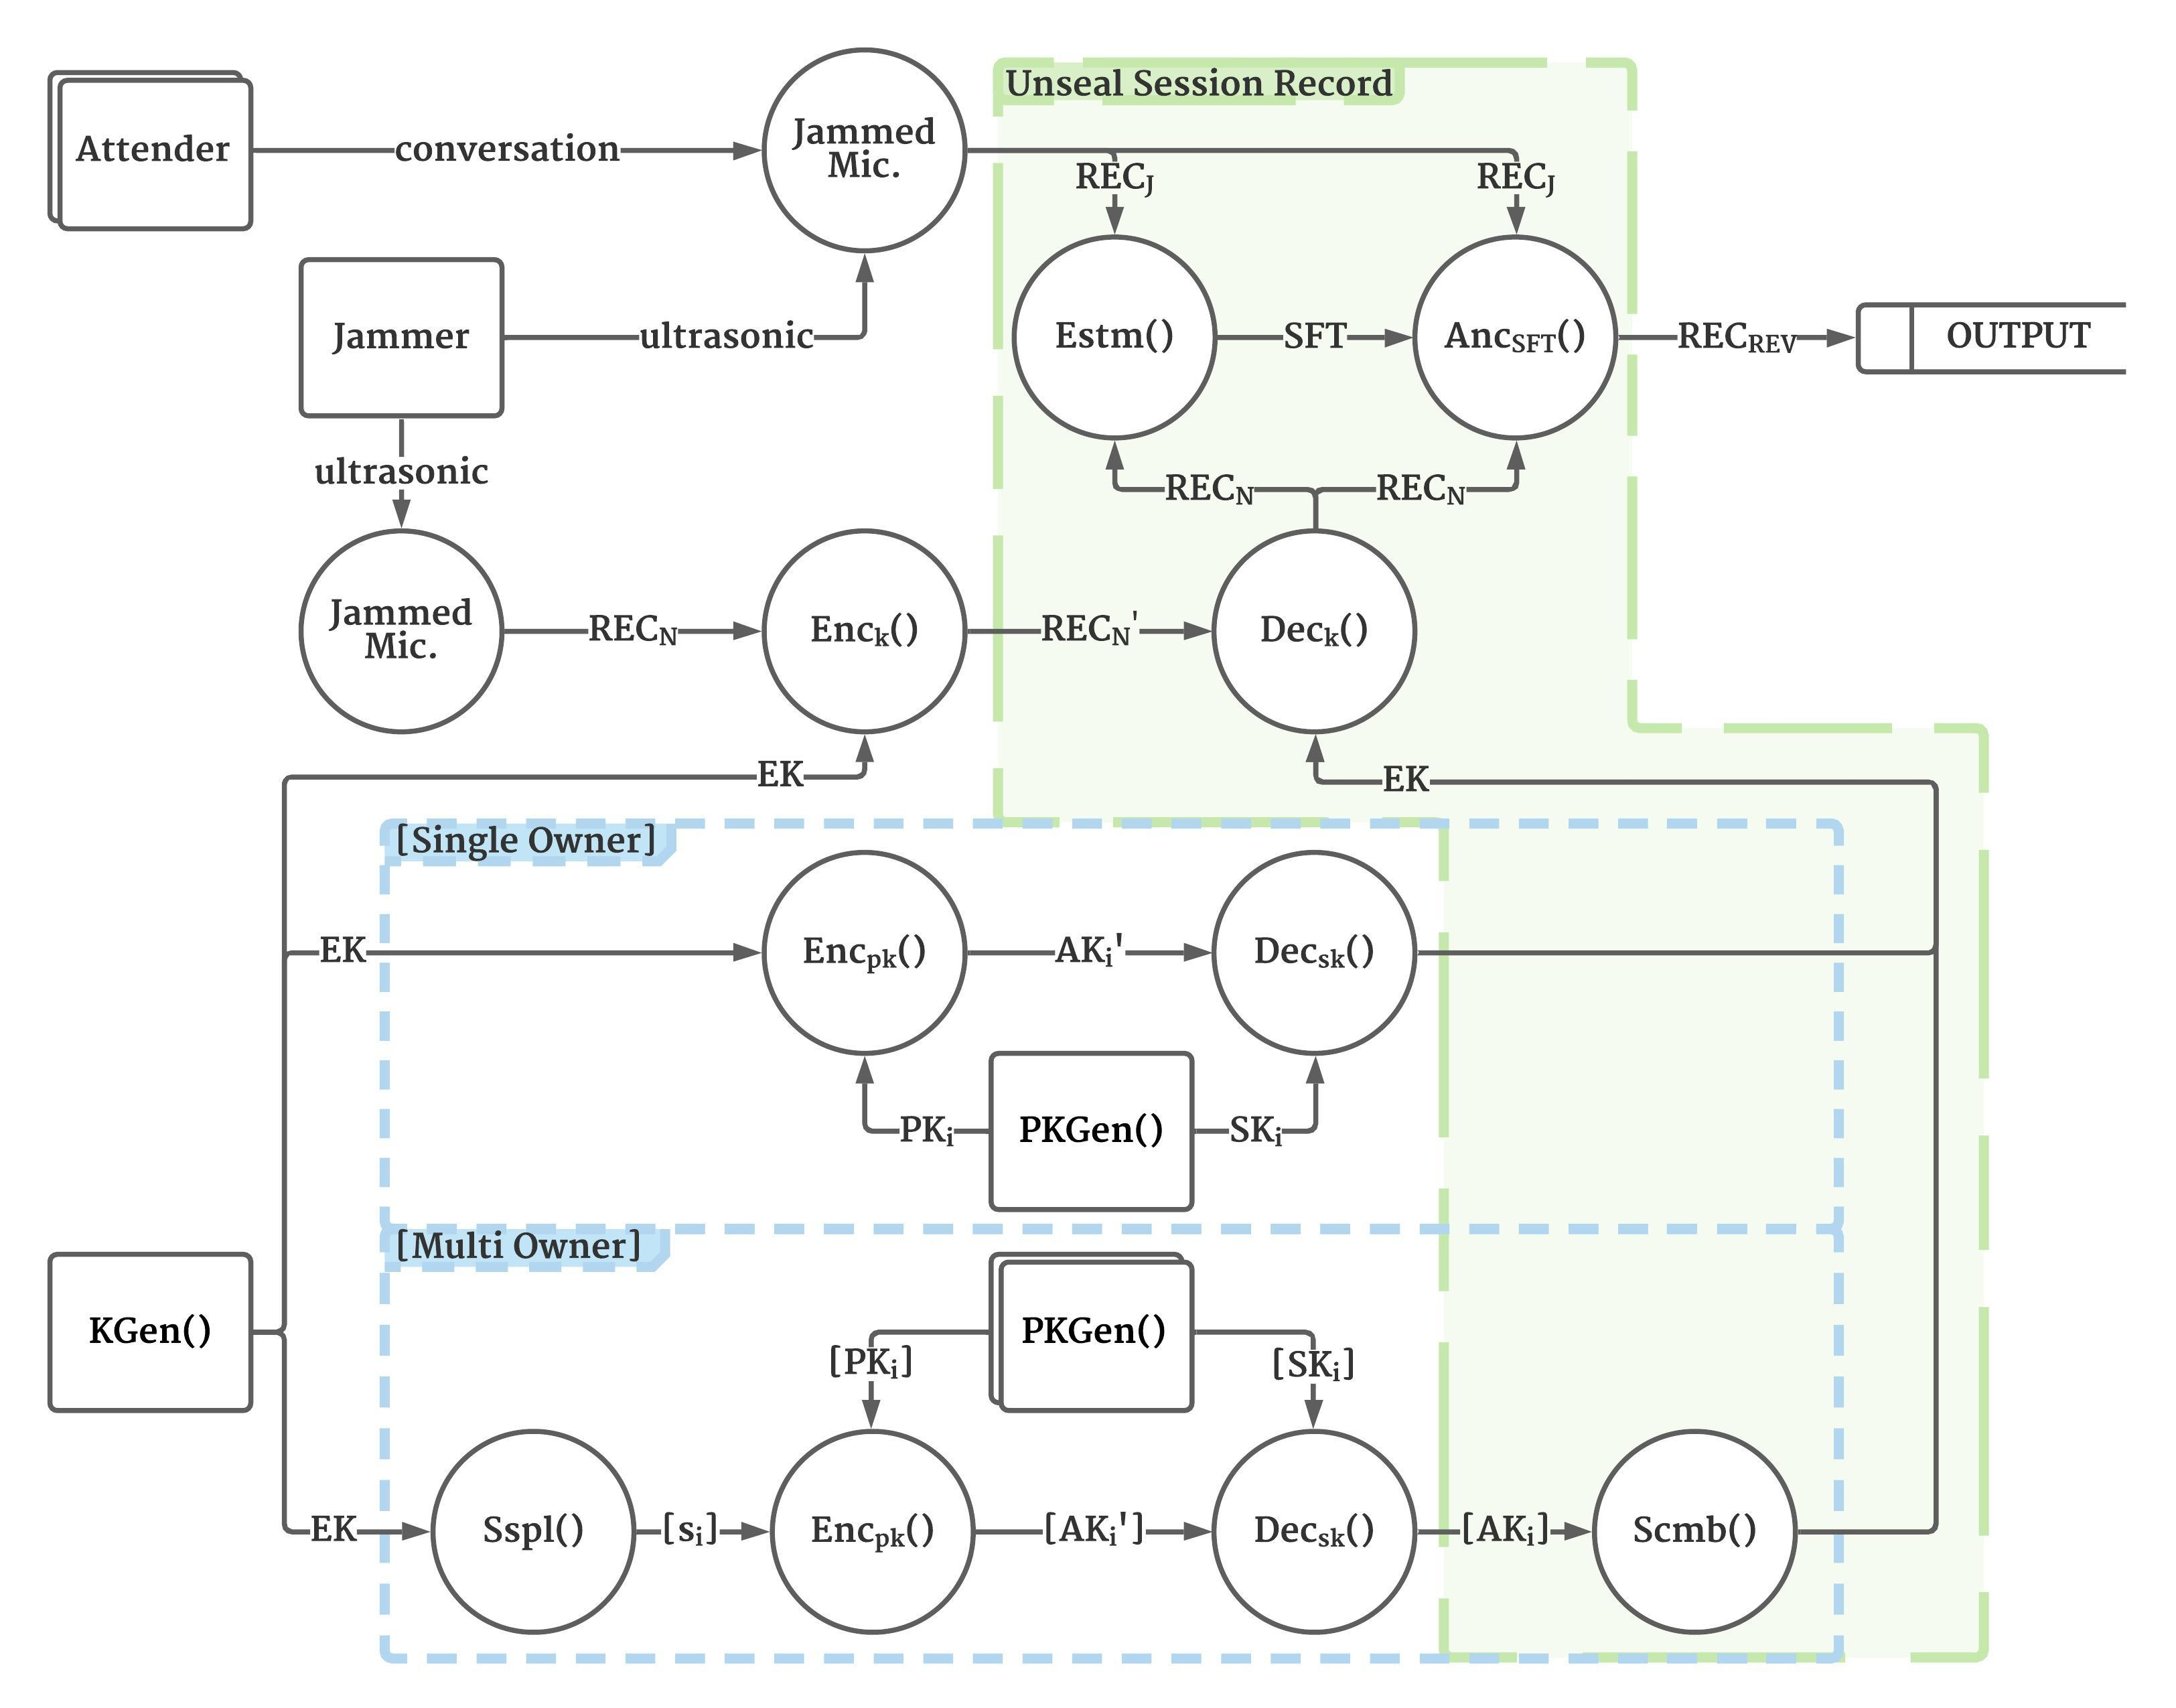
\includegraphics[width=1.0\textwidth]{system-data-flow}
    \caption{系統資料流程圖}\label{fig:system-data-flow}
\end{figure}


\subsubsection{唯密文攻擊}

    本研究假設,目前的技術發展現狀超音波麥克風干擾器可以對麥克風產生顯著的干擾效果\cite{chen2020demonstrating}。
本研究也透過實作嘗試復現 Yuxin Chen, Huiying Li 等人的成果 \cite{chen2020wearable},
並驗證其干擾效果,如實驗 \ref{subsec:exp-jammer}。
此超音波麥克風干擾機制原理為,將會談聲音內容(如會談對話)利用超音波麥克風干擾器對於麥克風的非線性響應輸出進行疊加,
因此可視為是對會談聲音內容利用干擾噪音進行串流加密。
與串流加密不同之處於,傳統串流加密的位元深度為 2,而對聲音進行串流加密的位元深度取決於取樣時後的量化深度,
常見 16位元有號整數或 32 位元浮點數。
因此若對於聲音的串流加密原始聲音與干擾聲音的信噪比不足,即便受干擾的聲音訊號已失真,
仍有可能於頻域分析或人耳聽聽感得出與原始聲音的關聯性。
透過實驗 \ref{subsec:exp-jammer} 結果得知,若信噪比達到約 $-22~dB$,
無法在沒有純超音波麥克風干擾器於麥克風的響應輸出(純噪音)之聲音記錄的情境下,有效還原原始聲音。
即意在會談聲音內容與干擾噪音信噪比達到約 $-22~dB$ 時,透過超音波噪音干擾對於麥克風產生的聲音紀錄內容進行串流加密,
且目前沒有已知有效方法可以對其進行唯密文攻擊(Ciphertext-only Attack,COA)。


\subsubsection{選擇明文攻擊}

    當超音波麥克風干擾器的干擾噪音與會談聲音內容進行疊加時視為串流加密時,此干擾噪音的產生原理如下。
首先透過隨機種子輸入偽隨機數產生於$24khz\sim26khz$之間的超音波,
接著透過麥克風對於超聲波干擾器的非線性響應輸出產生干擾噪音,此非線性響應輸出系統為不可知系統。
若攻擊者取得此加密機,透過構造一空白的會談聲音內容即可以取得在該離散時間內的純噪音。
純噪音可用於降噪還原受干擾的會談聲音紀錄,但僅限該離散時間內,
無法利用此離散時間內的純噪音獲取其他離散時間區間的明文。
原因為此干擾噪音為流密碼,其產生是透過偽隨機數產生器與不可知的非線性響應輸出系統,
在離散時間序列上有隨機性,因此無發透過片段流密碼得知其他流密碼進而獲取其他離散時間區間的明文,
因此可以有效抵禦選擇明文攻擊(Chosen-Plaintext Attack,CPA)。


\subsubsection{選擇密文攻擊}

    當受干擾的會談聲音紀錄與純超音波麥克風干擾器於麥克風的響應輸出(純噪音)之聲音記錄,
透過離散時間推估函數 \DEFfuncEstm{} 與 主動式噪音控制 \DEFfuncAnc{} 進行降噪還原時,
可視為是對會談聲音內容利用干擾噪音進行串流加密後,執行解密的方法。
與傳統的串流加密中的解密步驟不同,由於純噪音與受干擾的會談聲音紀錄中的干擾噪音並非完全相等僅高度相關,
因此若直接與離散時間序列上減去(抵銷干涉)純噪音,降噪還原效果不佳。
透過引入離散時間推估函數與主動式噪音控制來修正,如章節 \ref{sec:anc} \nameref{sec:anc},
此系統即可以有效還原出有效的會談聲音紀錄,作為會談聲音紀錄的以超音波麥克風干擾器的干擾噪音進行串流加密的解密方法,
如實驗 \ref{subsec:exp-snr-anc} \nameref{subsec:exp-snr-anc}。

    傳統的串流加密演算法無法抵禦選擇密文攻擊(Chosen-Ciphertext Attack,CCA)。
假設攻擊者可以取得解密機,透過惡意構造一皆為零的密文,即可獲得隱含於加密機中的金鑰。
當使用純超音波麥克風干擾器於麥克風的響應輸出(純噪音)之聲音記錄作為金鑰,
透過離散時間推估函數 \DEFfuncEstm{} 與 主動式噪音控制 \DEFfuncAnc{},對受干擾的會談聲音紀錄進行串流加密的解密時。
假設攻擊者取得此解密機且欲獲得隱含於加密機中的金鑰,透過構造一內容皆為零的惡意受干擾聲音紀錄作為密文進行攻擊,
無法如傳統的串流加密可獲得隱含於加密機中的金鑰。

    原因如下,基於章節 \ref{sec:anc} \nameref{sec:anc},為達到目標
$Min($\DEFmicRecREV $~-~$ \DEFmicConv $)~=~Min($ \DEFmicUSJ $~-~$ \DEFmicUSD $)$,
透過建立一遞移函數,使得 \DEFmicUSD 趨近於 \DEFmicUSJ,即可獲得 \DEFmicRecREV 趨近於 \DEFmicConv。
此時若受干擾聲音紀錄內容為零(\DEFmicRecJ $= 0$),
受干擾的會談聲音紀錄中不存在與純噪音高度相關的干擾噪音(\DEFmicUSJ $= 0$),
則代表為獲得最小 \DEFmicRecREV,需最小化遞移函數輸出 \DEFmicUSD 為零,其推導如下:

\begin{center}
\begin{tabularx}{0.55\textwidth} {>{\raggedright\arraybackslash}X}
    $Min($\DEFmicRecREV $~-~$ \DEFmicConv $)~=~Min($ \DEFmicUSJ $~-~$ \DEFmicUSD $)$ \\
    \DEFmicRecJ $~=~$ \DEFmicConv $~+~$ \DEFmicUSJ $~=~0$ \\
    \DEFmicConv $~=~$ \DEFmicUSJ $~=~0$ \\
    $Min($\DEFmicRecREV$)~=~Min(~-$\DEFmicUSD$)$ \\
\end{tabularx}
\end{center}

    因此當受干擾聲音紀錄內容為惡意構造皆為零的離散時間序列時,主動式噪音控制中的遞移函數傾向輸出為零,
因此無法透過惡意構造一內容皆為零的受干擾聲音紀錄,來獲得隱含於加密機中的金鑰。
因此相對於傳統串流加密法,基於超音波麥克風干擾器與主動式噪音控制的串流加密演算法,不受此攻擊手法影響。
且若搭配離散時間推估演算法,當受干擾的會談聲音紀錄中不存在與純噪音高度相關的干擾噪音,
此時即無法透過最小累計能量差在對齊點時顯著下降來找到對齊點。
故目前無已知有效方法可以對其進行選擇密文攻擊(Chosen-Ciphertext Attack,CCA)。

    前篇段落針對超音波麥克風干擾器與主動式噪音控制視為一串流加密系統進行安全性分析,並探討數個針對密碼系統的攻擊向量。
得出結論,在無純超音波麥克風干擾器於麥克風的響應輸出(純噪音)之聲音記錄作為解密金鑰時,
目前無已知有效的方法,可以還原出有效會談聲音紀錄。


\subsection{聲音記錄存取控制協定}

    接續段落將為聲音記錄存取控制協定進行安全性分析。


\subsubsection{系統脆弱點}

    分析章節 \ref{sec:protocol} \nameref{sec:protocol}可以得知,
解封金鑰 \DEFunsealKey 產生於\nameref{sec:protocol}的\nameref{subsec:protocol-init-create},
其產生者為系統角色解封伺服器 \DEFserver。
且於 \nameref{subsec:protocol-init-reg} 後於 \nameref{subsec:protocol-sessioning} 開始前錄音前,
於封伺服器 \DEFserver 銷毀。此時間區內,由於解封金鑰 \DEFunsealKey 以明文形式存在於解封伺服器 \DEFserver,
因此系統較為脆弱。例如:此時解封伺服器 \DEFserver 若遭受非預期的資訊安全風險,
導致以明文形式存在的解封金鑰 \DEFunsealKey 洩漏,則透過本研究所提出聲音記錄存取控制協定保護的此次會談的聲音紀錄,
可能因此而失去機密性。綜上所述,本研究所設計之\nameref{sec:protocol}可以確保,
在 \nameref{subsec:protocol-sessioning} 結束後,
直到成功解封 \nameref{subsec:protocol-unseal-access} 前,
有效的會談聲音紀錄 \DEFrecREV 保有機密性。


\subsubsection{中間人攻擊}

    本研究基於假設,系統各角色之間通訊為加密通道,提供通訊安全以保障資料的完整性、機密性。
透過引用目前的技術發展現狀的成熟技術,如傳輸層安全性協定(Transport Layer Security,TLS),
可以於通訊層就防止如竊聽攻擊(Sniffing attack)、
中間人攻擊(Man-in-the-middle attack,MITM) 的威脅 \cite{rfc5246}\cite{rfc8446}。


\subsubsection{冒名頂替攻擊}

    本研究所設計之系統將純噪音之聲音記錄 \DEFrecN 作為秘密保護,
透過解封金鑰 \DEFunsealKey 加密純噪音之聲音記錄 \DEFrecN,產生受加密保護的純噪音之聲音記錄 \DEFrecP。
當執行系統生命週期\nameref{subsec:unseal}時(圖 \ref{fig:system-data-flow} 中綠色虛線框處),
需要此解封金鑰 \DEFunsealKey 來解密受加密保護的純噪音之聲音記錄 \DEFrecP,
還原純噪音之聲音記錄 \DEFrecN 用於執行接續步驟以還原出有效的會談聲音紀錄 \DEFrecREV。

    會談主持者於註冊時會產生一非對稱是加密演算法的公開私密金鑰對。
並於註冊完成後根據會談主持者註冊人數是否為一或多人,
來判斷為單一會談主持者情境(\ref{fig:system-data-flow}藍色虛線框上半處)
或多會談主持者情境(\ref{fig:system-data-flow}藍色虛線框下半處),
應用此公開私密金鑰對達到目的將解封金鑰 \DEFunsealKey 的解密權限,轉交給會談主持者,
如 \ref{subsec:protocol-sessioning} \nameref{subsec:protocol-sessioning}。
協定中此階段為 Shamir's Secret Sharing \cite{shamir1979share}
與 RSA PKCS\#1 \cite{rfc8017} 的應用。
因次若將會談主持者妥善保管其私密金鑰 \DEFprivateKey,
基於 RSA \cite{rfc8017} 所保證的安全性,
冒名頂替攻擊(Impersonation attack) 無法形成威脅。


\section{相關系統比較}\label{sec:comparison}

    最近研究顯示,Lingkun Li 等人率先提出一套基於超音波麥克風干擾去與主動式噪音消除,
應用於防止未授權的對談錄音,並且於對談後還原\cite{li2020patronus}。
本研究所提出之「干擾保密與解密還原」與「會談聲音存取控制協定」的方法,
相較於 Lingkun Li 等人研究成果,不但降低演算法實作的複雜度,
且在提升系統可用性的同時,設計且實作了一套協定來滿足聲音記錄及存取情境。
比較如表 \ref{table:comparison} 。

\begin{longtable}{|c|c|c|c|c|c|}
    \caption{相關系統比較表}\label{table:comparison} \\
    \hline
    & 金鑰類型 & 金鑰大小 & 複雜度 & 實驗方式 & 干擾範圍 \\
    \hline
    \endfirsthead

    & 金鑰類型 & 金鑰大小 & 複雜度 & 實驗方式 & 干擾範圍 \\
    \hline
    \endhead

    \hline
    \endfoot

    \hline
    \endlastfoot

    本研究 &
    純噪音 &
    大 &
    簡單 &
    工程原型 &
    環形陣列 \\

    \hline

    Patronus\cite{li2020patronus} &
    頻率模式序列 &
    小 &
    複雜 &
    概念原型 &
    弧面反射 \\

\end{longtable}

    於 Lingkun Li 等人的研究成果 Patronus 中,
透過傳輸超音波麥克風干擾器產生干擾波的頻率模式序列與取樣率等元資料,組成作為降噪解密的金鑰。
原理為透過 Nirupam Roy 等人的研究成果 \cite{roy2017backdoor}\cite{roy2018inaudible} 中,
對於超音波於麥克風的非線性響應輸出的描述公式,嘗試模擬或還原原始超音波到麥克風取樣後的結果。
透過此轉換過程搭配主動式噪音控制即可消除被干擾的會談錄音中的干擾噪音。
於研究 Patronus 提到,根據實驗可能存在更高維度的因子在此非線性響應輸出中。
其變因包含,麥克風種類的不同(微電機、駐極體電容等),放大器與類比數位轉換器的不同,
因此轉換公式對於系統的描述也不同。
於本研究中,干擾保密與解密還原的過程,將超音波於麥克風的非線性響應輸出系統,視為一不可之系統。
透過直接記錄一段純超音波麥克風干擾器於麥克風的響應輸出(純噪音)之聲音記錄作為金鑰,
忽略此不可之系統的轉換過程,將純噪音之聲音記錄最為解密還原的金鑰。
此改變帶來的優點在於,因忽略不可之系統的變音,
因此對於不同種類的麥克風有著較高的相容性,且實作的複雜度也因此降低。
缺點在於,金鑰類型從隨機的頻率模式序列,替還為一離散時間序列的聲音樣本,因此金鑰所需的儲存容量較大。
